\documentclass[]{book}
\usepackage{lmodern}
\usepackage{amssymb,amsmath}
\usepackage{ifxetex,ifluatex}
\usepackage{fixltx2e} % provides \textsubscript
\ifnum 0\ifxetex 1\fi\ifluatex 1\fi=0 % if pdftex
  \usepackage[T1]{fontenc}
  \usepackage[utf8]{inputenc}
\else % if luatex or xelatex
  \ifxetex
    \usepackage{mathspec}
  \else
    \usepackage{fontspec}
  \fi
  \defaultfontfeatures{Ligatures=TeX,Scale=MatchLowercase}
\fi
% use upquote if available, for straight quotes in verbatim environments
\IfFileExists{upquote.sty}{\usepackage{upquote}}{}
% use microtype if available
\IfFileExists{microtype.sty}{%
\usepackage{microtype}
\UseMicrotypeSet[protrusion]{basicmath} % disable protrusion for tt fonts
}{}
\usepackage[margin=1in]{geometry}
\usepackage{hyperref}
\hypersetup{unicode=true,
            pdftitle={Data Analysis with Python Reference Book},
            pdfauthor={Boyan Angelov and Rick Scavetta},
            pdfborder={0 0 0},
            breaklinks=true}
\urlstyle{same}  % don't use monospace font for urls
\usepackage{natbib}
\bibliographystyle{apalike}
\usepackage{color}
\usepackage{fancyvrb}
\newcommand{\VerbBar}{|}
\newcommand{\VERB}{\Verb[commandchars=\\\{\}]}
\DefineVerbatimEnvironment{Highlighting}{Verbatim}{commandchars=\\\{\}}
% Add ',fontsize=\small' for more characters per line
\usepackage{framed}
\definecolor{shadecolor}{RGB}{248,248,248}
\newenvironment{Shaded}{\begin{snugshade}}{\end{snugshade}}
\newcommand{\AlertTok}[1]{\textcolor[rgb]{0.94,0.16,0.16}{#1}}
\newcommand{\AnnotationTok}[1]{\textcolor[rgb]{0.56,0.35,0.01}{\textbf{\textit{#1}}}}
\newcommand{\AttributeTok}[1]{\textcolor[rgb]{0.77,0.63,0.00}{#1}}
\newcommand{\BaseNTok}[1]{\textcolor[rgb]{0.00,0.00,0.81}{#1}}
\newcommand{\BuiltInTok}[1]{#1}
\newcommand{\CharTok}[1]{\textcolor[rgb]{0.31,0.60,0.02}{#1}}
\newcommand{\CommentTok}[1]{\textcolor[rgb]{0.56,0.35,0.01}{\textit{#1}}}
\newcommand{\CommentVarTok}[1]{\textcolor[rgb]{0.56,0.35,0.01}{\textbf{\textit{#1}}}}
\newcommand{\ConstantTok}[1]{\textcolor[rgb]{0.00,0.00,0.00}{#1}}
\newcommand{\ControlFlowTok}[1]{\textcolor[rgb]{0.13,0.29,0.53}{\textbf{#1}}}
\newcommand{\DataTypeTok}[1]{\textcolor[rgb]{0.13,0.29,0.53}{#1}}
\newcommand{\DecValTok}[1]{\textcolor[rgb]{0.00,0.00,0.81}{#1}}
\newcommand{\DocumentationTok}[1]{\textcolor[rgb]{0.56,0.35,0.01}{\textbf{\textit{#1}}}}
\newcommand{\ErrorTok}[1]{\textcolor[rgb]{0.64,0.00,0.00}{\textbf{#1}}}
\newcommand{\ExtensionTok}[1]{#1}
\newcommand{\FloatTok}[1]{\textcolor[rgb]{0.00,0.00,0.81}{#1}}
\newcommand{\FunctionTok}[1]{\textcolor[rgb]{0.00,0.00,0.00}{#1}}
\newcommand{\ImportTok}[1]{#1}
\newcommand{\InformationTok}[1]{\textcolor[rgb]{0.56,0.35,0.01}{\textbf{\textit{#1}}}}
\newcommand{\KeywordTok}[1]{\textcolor[rgb]{0.13,0.29,0.53}{\textbf{#1}}}
\newcommand{\NormalTok}[1]{#1}
\newcommand{\OperatorTok}[1]{\textcolor[rgb]{0.81,0.36,0.00}{\textbf{#1}}}
\newcommand{\OtherTok}[1]{\textcolor[rgb]{0.56,0.35,0.01}{#1}}
\newcommand{\PreprocessorTok}[1]{\textcolor[rgb]{0.56,0.35,0.01}{\textit{#1}}}
\newcommand{\RegionMarkerTok}[1]{#1}
\newcommand{\SpecialCharTok}[1]{\textcolor[rgb]{0.00,0.00,0.00}{#1}}
\newcommand{\SpecialStringTok}[1]{\textcolor[rgb]{0.31,0.60,0.02}{#1}}
\newcommand{\StringTok}[1]{\textcolor[rgb]{0.31,0.60,0.02}{#1}}
\newcommand{\VariableTok}[1]{\textcolor[rgb]{0.00,0.00,0.00}{#1}}
\newcommand{\VerbatimStringTok}[1]{\textcolor[rgb]{0.31,0.60,0.02}{#1}}
\newcommand{\WarningTok}[1]{\textcolor[rgb]{0.56,0.35,0.01}{\textbf{\textit{#1}}}}
\usepackage{longtable,booktabs}
\usepackage{graphicx,grffile}
\makeatletter
\def\maxwidth{\ifdim\Gin@nat@width>\linewidth\linewidth\else\Gin@nat@width\fi}
\def\maxheight{\ifdim\Gin@nat@height>\textheight\textheight\else\Gin@nat@height\fi}
\makeatother
% Scale images if necessary, so that they will not overflow the page
% margins by default, and it is still possible to overwrite the defaults
% using explicit options in \includegraphics[width, height, ...]{}
\setkeys{Gin}{width=\maxwidth,height=\maxheight,keepaspectratio}
\IfFileExists{parskip.sty}{%
\usepackage{parskip}
}{% else
\setlength{\parindent}{0pt}
\setlength{\parskip}{6pt plus 2pt minus 1pt}
}
\setlength{\emergencystretch}{3em}  % prevent overfull lines
\providecommand{\tightlist}{%
  \setlength{\itemsep}{0pt}\setlength{\parskip}{0pt}}
\setcounter{secnumdepth}{5}
% Redefines (sub)paragraphs to behave more like sections
\ifx\paragraph\undefined\else
\let\oldparagraph\paragraph
\renewcommand{\paragraph}[1]{\oldparagraph{#1}\mbox{}}
\fi
\ifx\subparagraph\undefined\else
\let\oldsubparagraph\subparagraph
\renewcommand{\subparagraph}[1]{\oldsubparagraph{#1}\mbox{}}
\fi

%%% Use protect on footnotes to avoid problems with footnotes in titles
\let\rmarkdownfootnote\footnote%
\def\footnote{\protect\rmarkdownfootnote}

%%% Change title format to be more compact
\usepackage{titling}

% Create subtitle command for use in maketitle
\newcommand{\subtitle}[1]{
  \posttitle{
    \begin{center}\large#1\end{center}
    }
}

\setlength{\droptitle}{-2em}

  \title{Data Analysis with Python Reference Book}
    \pretitle{\vspace{\droptitle}\centering\huge}
  \posttitle{\par}
    \author{Boyan Angelov and Rick Scavetta}
    \preauthor{\centering\large\emph}
  \postauthor{\par}
      \predate{\centering\large\emph}
  \postdate{\par}
    \date{2018-08-17}

\usepackage{booktabs}

\usepackage{amsthm}
\newtheorem{theorem}{Theorem}[chapter]
\newtheorem{lemma}{Lemma}[chapter]
\theoremstyle{definition}
\newtheorem{definition}{Definition}[chapter]
\newtheorem{corollary}{Corollary}[chapter]
\newtheorem{proposition}{Proposition}[chapter]
\theoremstyle{definition}
\newtheorem{example}{Example}[chapter]
\theoremstyle{definition}
\newtheorem{exercise}{Exercise}[chapter]
\theoremstyle{remark}
\newtheorem*{remark}{Remark}
\newtheorem*{solution}{Solution}
\begin{document}
\maketitle

{
\setcounter{tocdepth}{1}
\tableofcontents
}
\hypertarget{introductions}{%
\chapter{Introductions}\label{introductions}}

\hypertarget{set-up-your-software}{%
\section{Set up your software:}\label{set-up-your-software}}

Before running the commands in this book you should have the following
software locally installed:

\begin{itemize}
\tightlist
\item
  Python from \href{https://www.anaconda.com/download}{Anaconda}
\item
  Start the Anaconda Navigator and open up
  \href{https://jupyterlab.readthedocs.io/en/stable/}{Jupyter Lab}
\end{itemize}

\hypertarget{intro}{%
\chapter{ch 1: Basic Syntax and Types}\label{intro}}

\hypertarget{data-types}{%
\section{1.1 Data Types}\label{data-types}}

\begin{itemize}
\tightlist
\item
  int
\item
  float
\item
  bool: True and False
\item
  str
\end{itemize}

only use \texttt{=} for adding

\begin{Shaded}
\begin{Highlighting}[]
\NormalTok{x }\OperatorTok{=} \DecValTok{3}
\NormalTok{y }\OperatorTok{=} \FloatTok{0.5}
\NormalTok{z }\OperatorTok{=} \VariableTok{True}
\end{Highlighting}
\end{Shaded}

Types and classes

\begin{Shaded}
\begin{Highlighting}[]
\BuiltInTok{print}\NormalTok{(}\BuiltInTok{type}\NormalTok{(x))}
\end{Highlighting}
\end{Shaded}

\begin{verbatim}
## <class 'int'>
\end{verbatim}

\hypertarget{differences-in-handling-types}{%
\chapter{Differences in handling
types}\label{differences-in-handling-types}}

\begin{Shaded}
\begin{Highlighting}[]
\BuiltInTok{print}\NormalTok{(}\DecValTok{1} \OperatorTok{+} \DecValTok{1}\NormalTok{)}
\end{Highlighting}
\end{Shaded}

\begin{verbatim}
## 2
\end{verbatim}

\begin{Shaded}
\begin{Highlighting}[]
\BuiltInTok{print}\NormalTok{(}\StringTok{'1'} \OperatorTok{+} \StringTok{'1'}\NormalTok{)}
\end{Highlighting}
\end{Shaded}

\begin{verbatim}
## 11
\end{verbatim}

\begin{Shaded}
\begin{Highlighting}[]
\BuiltInTok{print}\NormalTok{(}\StringTok{'1'} \OperatorTok{*} \DecValTok{5}\NormalTok{)}
\end{Highlighting}
\end{Shaded}

\begin{verbatim}
## 11111
\end{verbatim}

\begin{Shaded}
\begin{Highlighting}[]
\BuiltInTok{print}\NormalTok{(}\StringTok{'1'} \StringTok{'1'}\NormalTok{)}
\end{Highlighting}
\end{Shaded}

\begin{verbatim}
## 11
\end{verbatim}

\hypertarget{containers---list-and-dictionaries}{%
\section{1.2 Containers - List and
Dictionaries}\label{containers---list-and-dictionaries}}

\hypertarget{lists}{%
\subsection{Lists}\label{lists}}

Holds heterogeneous information (e.g., {[}3, 2.718, True, `hello'{]})

\begin{Shaded}
\begin{Highlighting}[]
\NormalTok{l }\OperatorTok{=}\NormalTok{ [}\DecValTok{1}\NormalTok{, }\StringTok{'2'}\NormalTok{, }\VariableTok{True}\NormalTok{]}
\BuiltInTok{print}\NormalTok{(l)}
\end{Highlighting}
\end{Shaded}

\begin{verbatim}
## [1, '2', True]
\end{verbatim}

\begin{Shaded}
\begin{Highlighting}[]
\BuiltInTok{print}\NormalTok{(l[}\DecValTok{0}\NormalTok{]) }\CommentTok{# First value, use 0}
\end{Highlighting}
\end{Shaded}

\begin{verbatim}
## 1
\end{verbatim}

\begin{Shaded}
\begin{Highlighting}[]
\BuiltInTok{print}\NormalTok{(l[}\OperatorTok{-}\DecValTok{1}\NormalTok{]) }\CommentTok{# negative values, begin at end}
\end{Highlighting}
\end{Shaded}

\begin{verbatim}
## True
\end{verbatim}

\begin{Shaded}
\begin{Highlighting}[]
\NormalTok{l }\OperatorTok{=}\NormalTok{ [}\DecValTok{0}\NormalTok{, }\DecValTok{1}\NormalTok{, }\DecValTok{2}\NormalTok{, }\DecValTok{3}\NormalTok{, }\DecValTok{4}\NormalTok{]}
\BuiltInTok{print}\NormalTok{(l[}\DecValTok{0}\NormalTok{:}\DecValTok{3}\NormalTok{]) }\CommentTok{# first to third}
\end{Highlighting}
\end{Shaded}

\begin{verbatim}
## [0, 1, 2]
\end{verbatim}

\begin{Shaded}
\begin{Highlighting}[]
\BuiltInTok{print}\NormalTok{(l[}\DecValTok{0}\NormalTok{:}\DecValTok{5}\NormalTok{:}\DecValTok{2}\NormalTok{]) }\CommentTok{# step2}
\CommentTok{# Implicit}
\end{Highlighting}
\end{Shaded}

\begin{verbatim}
## [0, 2, 4]
\end{verbatim}

\begin{Shaded}
\begin{Highlighting}[]
\BuiltInTok{print}\NormalTok{(l[:}\DecValTok{3}\NormalTok{]) }\CommentTok{# first to third}
\end{Highlighting}
\end{Shaded}

\begin{verbatim}
## [0, 1, 2]
\end{verbatim}

\begin{Shaded}
\begin{Highlighting}[]
\BuiltInTok{print}\NormalTok{(l[}\DecValTok{1}\NormalTok{:]) }\CommentTok{# second to end}
\end{Highlighting}
\end{Shaded}

\begin{verbatim}
## [1, 2, 3, 4]
\end{verbatim}

\begin{Shaded}
\begin{Highlighting}[]
\BuiltInTok{print}\NormalTok{(l[::}\DecValTok{2}\NormalTok{]) }\CommentTok{# all, every second}
\CommentTok{# Explicit}
\end{Highlighting}
\end{Shaded}

\begin{verbatim}
## [0, 2, 4]
\end{verbatim}

\begin{Shaded}
\begin{Highlighting}[]
\BuiltInTok{print}\NormalTok{(l[}\DecValTok{0}\NormalTok{:}\DecValTok{3}\NormalTok{]) }\CommentTok{# }
\end{Highlighting}
\end{Shaded}

\begin{verbatim}
## [0, 1, 2]
\end{verbatim}

\begin{Shaded}
\begin{Highlighting}[]
\BuiltInTok{print}\NormalTok{(l[}\DecValTok{1}\NormalTok{:}\DecValTok{5}\NormalTok{]) }\CommentTok{# }
\end{Highlighting}
\end{Shaded}

\begin{verbatim}
## [1, 2, 3, 4]
\end{verbatim}

\begin{Shaded}
\begin{Highlighting}[]
\BuiltInTok{print}\NormalTok{(l[}\DecValTok{0}\NormalTok{:}\DecValTok{5}\NormalTok{:}\DecValTok{2}\NormalTok{])}
\end{Highlighting}
\end{Shaded}

\begin{verbatim}
## [0, 2, 4]
\end{verbatim}

\hypertarget{indexing}{%
\subsection{Indexing}\label{indexing}}

\begin{itemize}
\tightlist
\item
  Begins at zero
\item
  Negative values go in reverse
\item
  Left inclusive, right exclusive
\item
  Third value in index specifies step size
\item
  Can be implicit or explicit
\end{itemize}

\hypertarget{dictionaries}{%
\subsection{Dictionaries}\label{dictionaries}}

Lists are unlabelledm, but dictionaries provide key:value pairs using
\texttt{\{\}} and \texttt{:}.

\begin{Shaded}
\begin{Highlighting}[]
\NormalTok{d }\OperatorTok{=}\NormalTok{ \{}\StringTok{'int_value'}\NormalTok{:}\DecValTok{3}\NormalTok{, }
     \StringTok{'bool_value'}\NormalTok{:}\VariableTok{False}\NormalTok{, }
     \StringTok{'str_value'}\NormalTok{:}\StringTok{'hello'}\NormalTok{\}}
\BuiltInTok{print}\NormalTok{(d) }\CommentTok{# }
\end{Highlighting}
\end{Shaded}

\begin{verbatim}
## {'int_value': 3, 'bool_value': False, 'str_value': 'hello'}
\end{verbatim}

\begin{Shaded}
\begin{Highlighting}[]
\BuiltInTok{print}\NormalTok{(d[}\StringTok{'str_value'}\NormalTok{])}
\end{Highlighting}
\end{Shaded}

\begin{verbatim}
## hello
\end{verbatim}

Notice that the order when printing is different than in definition.
Order is not guaranteed! So don't rely on the printed order of the keys.

place key in the \texttt{{[}{]}} to extract that value.

\begin{Shaded}
\begin{Highlighting}[]
\NormalTok{l }\OperatorTok{=}\NormalTok{ [}\DecValTok{0}\NormalTok{, }\DecValTok{1}\NormalTok{, }\DecValTok{2}\NormalTok{, }\DecValTok{3}\NormalTok{, }\DecValTok{4}\NormalTok{]}
\NormalTok{d }\OperatorTok{=}\NormalTok{ \{}\StringTok{'int_value'}\NormalTok{:}\DecValTok{3}\NormalTok{, }\StringTok{'bool_value'}\NormalTok{:}\VariableTok{False}\NormalTok{, }\StringTok{'str_value'}\NormalTok{:}\StringTok{'hello'}\NormalTok{\}}
\BuiltInTok{print}\NormalTok{(}\BuiltInTok{len}\NormalTok{(l)) }\CommentTok{# }
\end{Highlighting}
\end{Shaded}

\begin{verbatim}
## 5
\end{verbatim}

\begin{Shaded}
\begin{Highlighting}[]
\BuiltInTok{print}\NormalTok{(}\BuiltInTok{len}\NormalTok{(d))}
\end{Highlighting}
\end{Shaded}

\begin{verbatim}
## 3
\end{verbatim}

\hypertarget{functions-methods-and-libraries}{%
\section{1.3 Functions, Methods, and
Libraries}\label{functions-methods-and-libraries}}

\begin{itemize}
\tightlist
\item
  Calling Functions
\item
  R and Python functions work the same
\item
  Python: Functions and Methods
\end{itemize}

\hypertarget{methods-vs-functions}{%
\subsection{Methods vs Functions}\label{methods-vs-functions}}

\begin{itemize}
\tightlist
\item
  python is an object-oriented programming language:

  \begin{itemize}
  \tightlist
  \item
    Attributes
  \item
    Methods
  \end{itemize}
\item
  Methods are functions that an object can call on itself
\item
  Functions are called on an object
\end{itemize}

\begin{Shaded}
\begin{Highlighting}[]
\NormalTok{l }\OperatorTok{=}\NormalTok{ [}\DecValTok{0}\NormalTok{, }\DecValTok{1}\NormalTok{, }\DecValTok{2}\NormalTok{, }\DecValTok{3}\NormalTok{, }\DecValTok{4}\NormalTok{]}
\BuiltInTok{len}\NormalTok{(l)   }\CommentTok{# call a function}
\end{Highlighting}
\end{Shaded}

But not this:

\begin{verbatim}
l.len()  # not a method
\end{verbatim}

e.g.~methods are functions that an object calls, whereas you pass
objects into functions.

i.e.~we pass \texttt{l} a list to the function \texttt{len()}, rather
than calling the method \texttt{len()} on \texttt{l} using the
\texttt{.}

\hypertarget{periods}{%
\subsection{periods}\label{periods}}

Periods, \texttt{.}, have very specific meanings and uses

You can't use a \texttt{.} in a variable or function name.

Uses:

Append a list: Call the append method on the list \texttt{l} using the
dot notation. So your not passing \texttt{l} to the \texttt{append()}
function, rather you're calling the \texttt{append()} method on list
\texttt{l}.

\begin{Shaded}
\begin{Highlighting}[]
\NormalTok{l }\OperatorTok{=}\NormalTok{ [}\DecValTok{1}\NormalTok{, }\StringTok{"2"}\NormalTok{, }\VariableTok{True}\NormalTok{]}
\NormalTok{l.append(}\StringTok{'appended value'}\NormalTok{)}
\BuiltInTok{print}\NormalTok{(l)}
\end{Highlighting}
\end{Shaded}

\begin{verbatim}
## [1, '2', True, 'appended value']
\end{verbatim}

Update a dictionary:

\begin{Shaded}
\begin{Highlighting}[]
\NormalTok{d }\OperatorTok{=}\NormalTok{ \{}\StringTok{'int_value'}\NormalTok{:}\DecValTok{3}\NormalTok{, }\StringTok{'bool_value'}\NormalTok{:}\VariableTok{False}\NormalTok{, }\StringTok{'str_value'}\NormalTok{:}\StringTok{'hello'}\NormalTok{\}}
\NormalTok{d.update(\{}\StringTok{'str_value'}\NormalTok{:}\StringTok{'new_value'}\NormalTok{, }\StringTok{'new_key'}\NormalTok{:}\StringTok{'new_value'}\NormalTok{\})}
\BuiltInTok{print}\NormalTok{(d)}
\end{Highlighting}
\end{Shaded}

\begin{verbatim}
## {'int_value': 3, 'bool_value': False, 'str_value': 'new_value', 'new_key': 'new_value'}
\end{verbatim}

Methods are special functions that belong to specific objects. e.g.~if
you try calling append on a dictionary object, you'll get an error
because the method append is not defined for a dictionary but it is
defined for a list.

\hypertarget{libraries}{%
\subsection{Libraries}\label{libraries}}

Arrays and data frame are not in Python by default. They come from numby
(array and matrix) and pandas (dataframe)

\begin{itemize}
\tightlist
\item
  Libraries provide more functionality
\item
  Arrays and dataframes are not built into Python
\item
  Arrays and matricies come from numpy
\item
  Dataframes come from pandas
\end{itemize}

use import to load the library, but use an alias with the as
\emph{keyword}.

\begin{Shaded}
\begin{Highlighting}[]
\ImportTok{import}\NormalTok{ numpy}
\CommentTok{# arr = numpy.loadtxt('my_file.csv', delimiter=',')}
\ImportTok{import}\NormalTok{ numpy }\ImportTok{as}\NormalTok{ np}
\CommentTok{# arr = np.loadtxt('my_file.csv', delimiter=',')}
\end{Highlighting}
\end{Shaded}

\begin{Shaded}
\begin{Highlighting}[]
\ImportTok{import}\NormalTok{ pandas }\ImportTok{as}\NormalTok{ pd}
\CommentTok{# df = pd.read_csv('my_file.csv')}
\CommentTok{# df.head()}
\end{Highlighting}
\end{Shaded}

\hypertarget{extra}{%
\section{Extra}\label{extra}}

Find out where your packages are. In python execute:

\begin{Shaded}
\begin{Highlighting}[]
\ImportTok{import}\NormalTok{ pandas}
\ImportTok{import}\NormalTok{ os}
\NormalTok{path }\OperatorTok{=}\NormalTok{ os.path.dirname(pandas.}\VariableTok{__file__}\NormalTok{)}
\BuiltInTok{print}\NormalTok{(path)}
\end{Highlighting}
\end{Shaded}

\begin{verbatim}
## /anaconda3/lib/python3.6/site-packages/pandas
\end{verbatim}

\begin{Shaded}
\begin{Highlighting}[]
\ImportTok{import}\NormalTok{ sys}
\BuiltInTok{print}\NormalTok{(sys.version)}
\end{Highlighting}
\end{Shaded}

\begin{verbatim}
## 3.6.4 |Anaconda, Inc.| (default, Jan 16 2018, 12:06:34) 
## [GCC 4.2.1 Compatible Clang 4.0.1 (tags/RELEASE_401/final)]
\end{verbatim}

\begin{Shaded}
\begin{Highlighting}[]
\BuiltInTok{print}\NormalTok{(sys.executable)}
\end{Highlighting}
\end{Shaded}

\begin{verbatim}
## /anaconda3/bin/python
\end{verbatim}

\begin{Shaded}
\begin{Highlighting}[]
\KeywordTok{print}\NormalTok{(}\KeywordTok{system}\NormalTok{(}\StringTok{"which python"}\NormalTok{))}
\end{Highlighting}
\end{Shaded}

\begin{verbatim}
## [1] 0
\end{verbatim}

\hypertarget{ch-2}{%
\chapter{ch 2}\label{ch-2}}

\hypertarget{if-statements-and-loops}{%
\section{2.1 If statements and Loops}\label{if-statements-and-loops}}

\emph{Whitespace and indentation is a fundamental part of writing python
code and is not optional}.

i.e.~you define code blocks with indentations. Use 4 spaces to indent
code

\begin{Shaded}
\begin{Highlighting}[]
\ControlFlowTok{if} \DecValTok{5} \OperatorTok{==} \DecValTok{5}\NormalTok{:}
    \BuiltInTok{print}\NormalTok{(}\StringTok{'True'}\NormalTok{)}
    
\end{Highlighting}
\end{Shaded}

\begin{verbatim}
## True
\end{verbatim}

Everything in the indented code is executed in python. That's like
\texttt{\{\}} in R

\texttt{elif} and \texttt{else}:

\begin{Shaded}
\begin{Highlighting}[]
\NormalTok{val }\OperatorTok{=} \DecValTok{2}
\ControlFlowTok{if}\NormalTok{ val }\OperatorTok{==} \DecValTok{1}\NormalTok{:}
    \BuiltInTok{print}\NormalTok{(}\StringTok{'snap'}\NormalTok{)}
\ControlFlowTok{elif}\NormalTok{ val }\OperatorTok{==} \DecValTok{2}\NormalTok{:}
    \BuiltInTok{print}\NormalTok{(}\StringTok{'crackle'}\NormalTok{)}
\ControlFlowTok{else}\NormalTok{:}
    \BuiltInTok{print}\NormalTok{(}\StringTok{'pop'}\NormalTok{)}
\end{Highlighting}
\end{Shaded}

\begin{verbatim}
## crackle
\end{verbatim}

for loops:

\begin{Shaded}
\begin{Highlighting}[]
\NormalTok{num_val }\OperatorTok{=}\NormalTok{ [}\DecValTok{1}\NormalTok{, }\DecValTok{2}\NormalTok{, }\DecValTok{3}\NormalTok{, }\DecValTok{4}\NormalTok{]}
\ControlFlowTok{for}\NormalTok{ value }\KeywordTok{in}\NormalTok{ num_val:}
    \BuiltInTok{print}\NormalTok{(value)}
\end{Highlighting}
\end{Shaded}

\begin{verbatim}
## 1
## 2
## 3
## 4
\end{verbatim}

\hypertarget{functions}{%
\section{2.2 Functions}\label{functions}}

\hypertarget{writing-your-own-functions}{%
\subsection{2.2.1 Writing your own
functions:}\label{writing-your-own-functions}}

use the \texttt{def} keyword in Python. The body of the function is
indented. The \texttt{return} statement is necessary! The last line is
not automatically returned.

\begin{Shaded}
\begin{Highlighting}[]
\KeywordTok{def}\NormalTok{ my_mean(x, y):}
\NormalTok{    num }\OperatorTok{=}\NormalTok{ x }\OperatorTok{+}\NormalTok{ y}
\NormalTok{    dem }\OperatorTok{=} \DecValTok{2}
    \ControlFlowTok{return}\NormalTok{ num }\OperatorTok{/}\NormalTok{ dem}
\BuiltInTok{print}\NormalTok{(my_mean(}\DecValTok{10}\NormalTok{, }\DecValTok{20}\NormalTok{))}
\end{Highlighting}
\end{Shaded}

\begin{verbatim}
## 15.0
\end{verbatim}

\hypertarget{functions-can-call-other-functions}{%
\subsection{2.2.2 Functions can call other
functions:}\label{functions-can-call-other-functions}}

\begin{Shaded}
\begin{Highlighting}[]
\KeywordTok{def}\NormalTok{ my_sq(x):}
    \ControlFlowTok{return}\NormalTok{ x }\OperatorTok{**} \DecValTok{2}
    
\KeywordTok{def}\NormalTok{ my_sq_mean(y, z):}
    \ControlFlowTok{return}\NormalTok{ (my_sq(y) }\OperatorTok{+}\NormalTok{ my_sq(z)) }\OperatorTok{/} \DecValTok{2}
    
\BuiltInTok{print}\NormalTok{(my_sq_mean(}\DecValTok{10}\NormalTok{, }\DecValTok{12}\NormalTok{))}
\end{Highlighting}
\end{Shaded}

\begin{verbatim}
## 122.0
\end{verbatim}

\hypertarget{anonymous-and-lambda-functions}{%
\subsection{2.2.3 Anonymous and lambda
functions}\label{anonymous-and-lambda-functions}}

In Python, use the \texttt{lambda} keyword to make a lambda functions
with the apply method (see later):

\begin{Shaded}
\begin{Highlighting}[]
\KeywordTok{def}\NormalTok{ add_1(x):}
    \ControlFlowTok{return}\NormalTok{ x }\OperatorTok{+} \DecValTok{1}
    
\NormalTok{a1_lam }\OperatorTok{=} \KeywordTok{lambda}\NormalTok{ x: x }\OperatorTok{+} \DecValTok{1}
\BuiltInTok{print}\NormalTok{(a1_lam(}\DecValTok{3}\NormalTok{))}
\end{Highlighting}
\end{Shaded}

\begin{verbatim}
## 4
\end{verbatim}

You can also save a lambda funcion.

\hypertarget{comprehensions}{%
\section{2.3 Comprehensions}\label{comprehensions}}

One of the most common tasks you'll perform when cleaning or summarising
data is to iterate over a list, apply some function or perform some
calculation on each element and then return the result as a new list.

\hypertarget{list-comprehensions}{%
\subsection{2.3.1 List comprehensions}\label{list-comprehensions}}

Comprehensions are loops:

\begin{itemize}
\tightlist
\item
  Iterate (loop) through a list
\item
  Perform some function
\item
  Append results into a new list
\end{itemize}

Open a \texttt{{[}{]}} and write the body of your \texttt{for\ loop}
first then write the for statement to iterate over data. No \texttt{:}
at the end!

\texttt{for\ loop}:

\begin{Shaded}
\begin{Highlighting}[]
\NormalTok{data }\OperatorTok{=}\NormalTok{ [}\DecValTok{1}\NormalTok{, }\DecValTok{2}\NormalTok{, }\DecValTok{3}\NormalTok{, }\DecValTok{4}\NormalTok{, }\DecValTok{5}\NormalTok{]}
\NormalTok{new }\OperatorTok{=}\NormalTok{ []}
\ControlFlowTok{for}\NormalTok{ x }\KeywordTok{in}\NormalTok{ data:}
\NormalTok{    new.append(x}\OperatorTok{**}\DecValTok{2}\NormalTok{)}
\BuiltInTok{print}\NormalTok{(new)}
\end{Highlighting}
\end{Shaded}

\begin{verbatim}
## [1, 4, 9, 16, 25]
\end{verbatim}

Comprehension:

\begin{Shaded}
\begin{Highlighting}[]
\NormalTok{data }\OperatorTok{=}\NormalTok{ [}\DecValTok{1}\NormalTok{, }\DecValTok{2}\NormalTok{, }\DecValTok{3}\NormalTok{, }\DecValTok{4}\NormalTok{, }\DecValTok{5}\NormalTok{]}
\NormalTok{new }\OperatorTok{=}\NormalTok{ [x}\OperatorTok{**}\DecValTok{2} \ControlFlowTok{for}\NormalTok{ x }\KeywordTok{in}\NormalTok{ data]}
\BuiltInTok{print}\NormalTok{(new)}
\end{Highlighting}
\end{Shaded}

\begin{verbatim}
## [1, 4, 9, 16, 25]
\end{verbatim}

\hypertarget{dictionary-comprehensions}{%
\subsection{2.3.3 Dictionary
comprehensions}\label{dictionary-comprehensions}}

Result is a dictionary, so you need to create a key:value pair. Use
\texttt{\{\}} here

\texttt{for\ loop}:

\begin{Shaded}
\begin{Highlighting}[]
\NormalTok{data }\OperatorTok{=}\NormalTok{ [}\DecValTok{1}\NormalTok{, }\DecValTok{2}\NormalTok{, }\DecValTok{3}\NormalTok{, }\DecValTok{4}\NormalTok{, }\DecValTok{5}\NormalTok{]}
\NormalTok{new }\OperatorTok{=}\NormalTok{ \{\}}
\ControlFlowTok{for}\NormalTok{ x }\KeywordTok{in}\NormalTok{ data:}
\NormalTok{    new[x] }\OperatorTok{=}\NormalTok{ x}\OperatorTok{**}\DecValTok{2}
\BuiltInTok{print}\NormalTok{(new)}
\end{Highlighting}
\end{Shaded}

\begin{verbatim}
## {1: 1, 2: 4, 3: 9, 4: 16, 5: 25}
\end{verbatim}

Comprehension:

\begin{Shaded}
\begin{Highlighting}[]
\NormalTok{data }\OperatorTok{=}\NormalTok{ [}\DecValTok{1}\NormalTok{, }\DecValTok{2}\NormalTok{, }\DecValTok{3}\NormalTok{, }\DecValTok{4}\NormalTok{, }\DecValTok{5}\NormalTok{]}
\NormalTok{new }\OperatorTok{=}\NormalTok{ \{x: x}\OperatorTok{**}\DecValTok{2} \ControlFlowTok{for}\NormalTok{ x }\KeywordTok{in}\NormalTok{ data\}}
\BuiltInTok{print}\NormalTok{(new)}
\end{Highlighting}
\end{Shaded}

\begin{verbatim}
## {1: 1, 2: 4, 3: 9, 4: 16, 5: 25}
\end{verbatim}

\hypertarget{alternatives-to-for-loops}{%
\subsection{2.3.4 Alternatives to for
loops}\label{alternatives-to-for-loops}}

\begin{itemize}
\tightlist
\item
  \texttt{for\ loop} to iterate
\item
  R: sapply, lapply, apply functions
\item
  Python: map function (here) and apply method
\end{itemize}

\texttt{map()} takes the name of the function as the first argument and
a list of values as the second. The specified funtion is applied to all
the elements in the second argument, one at a time, like
\texttt{sapply()} and \texttt{lapply()} in R. The result is a
\texttt{map} object, so you need to convert it to a \texttt{list} to
view it.

\texttt{for\ loop}:

\begin{Shaded}
\begin{Highlighting}[]
\KeywordTok{def}\NormalTok{ sq(x):}
    \ControlFlowTok{return}\NormalTok{ x}\OperatorTok{**}\DecValTok{2}
\NormalTok{l }\OperatorTok{=}\NormalTok{ [}\DecValTok{1}\NormalTok{, }\DecValTok{2}\NormalTok{, }\DecValTok{3}\NormalTok{]}
\ControlFlowTok{for}\NormalTok{ i }\KeywordTok{in}\NormalTok{ l:}
    \BuiltInTok{print}\NormalTok{(sq(i))}
    
\end{Highlighting}
\end{Shaded}

\begin{verbatim}
## 1
## 4
## 9
\end{verbatim}

\texttt{map()}

\begin{Shaded}
\begin{Highlighting}[]
\BuiltInTok{map}\NormalTok{(sq, l)}
\BuiltInTok{print}\NormalTok{(}\BuiltInTok{list}\NormalTok{(}\BuiltInTok{map}\NormalTok{(sq, l)))}
\end{Highlighting}
\end{Shaded}

\begin{verbatim}
## [1, 4, 9]
\end{verbatim}

\hypertarget{ch-3-selecting-data-in-pandas}{%
\chapter{Ch 3: Selecting Data in
Pandas}\label{ch-3-selecting-data-in-pandas}}

\hypertarget{data-frames---2d}{%
\section{3.1.1 Data frames - 2D}\label{data-frames---2d}}

You can pass a dictionary to a \texttt{pd.DataFrame()} function. Index
specifies the row names.

\begin{Shaded}
\begin{Highlighting}[]
\NormalTok{df =}\StringTok{ }\KeywordTok{data.frame}\NormalTok{(}\DataTypeTok{A =} \DecValTok{1}\OperatorTok{:}\DecValTok{3}\NormalTok{,}
                \DataTypeTok{B =} \DecValTok{4}\OperatorTok{:}\DecValTok{6}\NormalTok{,}
                \DataTypeTok{C =} \DecValTok{7}\OperatorTok{:}\DecValTok{9}\NormalTok{,}
                \DataTypeTok{row.names =} \KeywordTok{c}\NormalTok{(}\StringTok{"x"}\NormalTok{, }\StringTok{"y"}\NormalTok{, }\StringTok{"z"}\NormalTok{))}
\end{Highlighting}
\end{Shaded}

\begin{Shaded}
\begin{Highlighting}[]
\ImportTok{import}\NormalTok{ pandas }\ImportTok{as}\NormalTok{ pd}
\NormalTok{df }\OperatorTok{=}\NormalTok{ pd.DataFrame(\{}
            \StringTok{'A'}\NormalTok{: [}\DecValTok{1}\NormalTok{, }\DecValTok{2}\NormalTok{, }\DecValTok{3}\NormalTok{],}
            \StringTok{'B'}\NormalTok{: [}\DecValTok{4}\NormalTok{, }\DecValTok{5}\NormalTok{, }\DecValTok{6}\NormalTok{], }
            \StringTok{'C'}\NormalTok{: [}\DecValTok{7}\NormalTok{, }\DecValTok{8}\NormalTok{, }\DecValTok{9}\NormalTok{]\}, }
\NormalTok{            index }\OperatorTok{=}\NormalTok{ [}\StringTok{'x'}\NormalTok{, }\StringTok{'y'}\NormalTok{, }\StringTok{'z'}\NormalTok{])}
\BuiltInTok{print}\NormalTok{(df)}
\end{Highlighting}
\end{Shaded}

\begin{verbatim}
##    A  B  C
## x  1  4  7
## y  2  5  8
## z  3  6  9
\end{verbatim}

Select columns:

\begin{Shaded}
\begin{Highlighting}[]
\NormalTok{df[}\StringTok{'A'}\NormalTok{]}
\NormalTok{df.A}
\NormalTok{df[[}\StringTok{'A'}\NormalTok{, }\StringTok{'B'}\NormalTok{]]}
\end{Highlighting}
\end{Shaded}

Subset rows by index position (iloc)

\begin{Shaded}
\begin{Highlighting}[]
\NormalTok{df}
\NormalTok{df.iloc[}\DecValTok{0}\NormalTok{] }\CommentTok{# First row}
\NormalTok{df.iloc[[}\DecValTok{0}\NormalTok{, }\DecValTok{1}\NormalTok{]] }\CommentTok{# a list of rows, the first two rows}
\end{Highlighting}
\end{Shaded}

\begin{Shaded}
\begin{Highlighting}[]
\NormalTok{df.iloc[}\DecValTok{0}\NormalTok{, :] }\CommentTok{# all columns, : after the comma}
\NormalTok{df.iloc[[}\DecValTok{0}\NormalTok{, }\DecValTok{1}\NormalTok{], :]}
\end{Highlighting}
\end{Shaded}

Subsetting rows by label (loc)

\begin{Shaded}
\begin{Highlighting}[]
\NormalTok{df.loc[}\StringTok{'x'}\NormalTok{] }\CommentTok{# The xth row}
\NormalTok{df.loc[[}\StringTok{'x'}\NormalTok{, }\StringTok{'y'}\NormalTok{]] }\CommentTok{# The xth and yth row}
\end{Highlighting}
\end{Shaded}

Both rows and columns

\begin{Shaded}
\begin{Highlighting}[]
\NormalTok{df.loc[}\StringTok{'x'}\NormalTok{, }\StringTok{'A'}\NormalTok{]}
\NormalTok{df.loc[[}\StringTok{'x'}\NormalTok{, }\StringTok{'y'}\NormalTok{], [}\StringTok{'A'}\NormalTok{, }\StringTok{'B'}\NormalTok{]]}
\end{Highlighting}
\end{Shaded}

Conditional subsetting

\begin{Shaded}
\begin{Highlighting}[]
\NormalTok{df[df.A }\OperatorTok{==} \DecValTok{3}\NormalTok{]}
\NormalTok{df[(df.A }\OperatorTok{==} \DecValTok{3}\NormalTok{) }\OperatorTok{|}\NormalTok{ (df.B }\OperatorTok{==} \DecValTok{4}\NormalTok{)]}
\end{Highlighting}
\end{Shaded}

\hypertarget{attributes}{%
\section{3.1.2 Attributes}\label{attributes}}

Shape is an attribute, so no \texttt{()}:

\begin{Shaded}
\begin{Highlighting}[]
\NormalTok{df.shape}
\end{Highlighting}
\end{Shaded}

NOT a functon

\begin{Shaded}
\begin{Highlighting}[]
\NormalTok{df.shape()}
\end{Highlighting}
\end{Shaded}

\hypertarget{data-types-1}{%
\section{3.2.1 Data Types}\label{data-types-1}}

type returns the type of an object. Data frames have more info.

\begin{Shaded}
\begin{Highlighting}[]
\KeywordTok{str}\NormalTok{(df)}
\end{Highlighting}
\end{Shaded}

\begin{verbatim}
## 'data.frame':    3 obs. of  3 variables:
##  $ A: int  1 2 3
##  $ B: int  4 5 6
##  $ C: int  7 8 9
\end{verbatim}

\begin{Shaded}
\begin{Highlighting}[]
\NormalTok{df.info()}
\end{Highlighting}
\end{Shaded}

\begin{verbatim}
## <class 'pandas.core.frame.DataFrame'>
## Index: 3 entries, x to z
## Data columns (total 3 columns):
## A    3 non-null int64
## B    3 non-null int64
## C    3 non-null int64
## dtypes: int64(3)
## memory usage: 176.0+ bytes
\end{verbatim}

\hypertarget{change-data-types}{%
\subsection{3.2.2 Change data types:}\label{change-data-types}}

\begin{Shaded}
\begin{Highlighting}[]
\NormalTok{df}\OperatorTok{$}\NormalTok{A <-}\StringTok{ }\KeywordTok{as.character}\NormalTok{(df}\OperatorTok{$}\NormalTok{A)}
\KeywordTok{str}\NormalTok{(df)}
\end{Highlighting}
\end{Shaded}

\begin{verbatim}
## 'data.frame':    3 obs. of  3 variables:
##  $ A: chr  "1" "2" "3"
##  $ B: int  4 5 6
##  $ C: int  7 8 9
\end{verbatim}

\begin{Shaded}
\begin{Highlighting}[]
\NormalTok{df[}\StringTok{'A'}\NormalTok{] }\OperatorTok{=}\NormalTok{ df[}\StringTok{'A'}\NormalTok{].astype(}\BuiltInTok{str}\NormalTok{)}
\NormalTok{df.info()}
\end{Highlighting}
\end{Shaded}

\begin{verbatim}
## <class 'pandas.core.frame.DataFrame'>
## Index: 3 entries, x to z
## Data columns (total 3 columns):
## A    3 non-null object
## B    3 non-null int64
## C    3 non-null int64
## dtypes: int64(2), object(1)
## memory usage: 176.0+ bytes
\end{verbatim}

Type \texttt{object} means \texttt{string}. Access built-in string
methods with str accessor

\hypertarget{accessors}{%
\subsection{3.2.3 Accessors}\label{accessors}}

\hypertarget{string-accessor}{%
\subsubsection{3.2.3.1 String Accessor}\label{string-accessor}}

e.g.~strip removed leading and trailing whitespece

\begin{Shaded}
\begin{Highlighting}[]
\NormalTok{df }\OperatorTok{=}\NormalTok{ pd.DataFrame(\{}\StringTok{'name'}\NormalTok{: [}\StringTok{'Daniel  '}\NormalTok{,}\StringTok{'  Eric'}\NormalTok{, }\StringTok{'  Julia  '}\NormalTok{]\})}
\NormalTok{df[}\StringTok{'name_strip'}\NormalTok{] }\OperatorTok{=}\NormalTok{ df[}\StringTok{'name'}\NormalTok{].}\BuiltInTok{str}\NormalTok{.strip()}
\NormalTok{df}
\end{Highlighting}
\end{Shaded}

\hypertarget{categorical-accessor}{%
\subsubsection{3.2.3.1 Categorical
Accessor}\label{categorical-accessor}}

Like factors in R

\begin{Shaded}
\begin{Highlighting}[]
\NormalTok{df }\OperatorTok{=}\NormalTok{ pd.DataFrame(\{}\StringTok{'name'}\NormalTok{: [}\StringTok{'Daniel'}\NormalTok{,}\StringTok{'Eric'}\NormalTok{, }\StringTok{'Julia'}\NormalTok{],}
                   \StringTok{'gender'}\NormalTok{:[}\StringTok{'Male'}\NormalTok{, }\StringTok{'Male'}\NormalTok{, }\StringTok{'Female'}\NormalTok{]\})}
\NormalTok{df[}\StringTok{'gender_cat'}\NormalTok{] }\OperatorTok{=}\NormalTok{ df[}\StringTok{'gender'}\NormalTok{].astype(}\StringTok{'category'}\NormalTok{) }
\end{Highlighting}
\end{Shaded}

See the categories (levels in R) by calling the \texttt{cat} accessor
and the \texttt{categories} attribute on the column. Use the
\texttt{codes} attribute to get the codes.

\begin{Shaded}
\begin{Highlighting}[]
\NormalTok{df[}\StringTok{'gender_cat'}\NormalTok{].cat.categories}
\NormalTok{df.gender_cat.cat.codes}
\end{Highlighting}
\end{Shaded}

\hypertarget{date-accessor}{%
\subsubsection{3.2.3.3 Date Accessor}\label{date-accessor}}

Dates: use the \texttt{to\_datetime()} function

\begin{Shaded}
\begin{Highlighting}[]
\NormalTok{df }\OperatorTok{=}\NormalTok{ pd.DataFrame(\{}\StringTok{'name'}\NormalTok{: [}\StringTok{'Rosaline Franklin'}\NormalTok{, }\StringTok{'William Gosset'}\NormalTok{], }
                   \StringTok{'born'}\NormalTok{: [}\StringTok{'1920-07-25'}\NormalTok{, }\StringTok{'1876-06-13'}\NormalTok{]\})}
\NormalTok{df[}\StringTok{'born_dt'}\NormalTok{] }\OperatorTok{=}\NormalTok{ pd.to_datetime(df[}\StringTok{'born'}\NormalTok{])}
\end{Highlighting}
\end{Shaded}

Similar to strings and categorical values, you can access date
components with the \texttt{dt} accessor

\begin{Shaded}
\begin{Highlighting}[]
\NormalTok{df[}\StringTok{'born_dt'}\NormalTok{].dt.day}
\NormalTok{df[}\StringTok{'born_dt'}\NormalTok{].dt.month}
\NormalTok{df[}\StringTok{'born_dt'}\NormalTok{].dt.year}
\end{Highlighting}
\end{Shaded}

\hypertarget{advanced-pandas}{%
\section{3.3 Advanced Pandas}\label{advanced-pandas}}

\hypertarget{missing-data}{%
\subsection{3.3.1 Missing data}\label{missing-data}}

\begin{itemize}
\tightlist
\item
  \texttt{NaN} missing values from from numpy
\item
  \texttt{np.NaN}, \texttt{np.NAN}, \texttt{np.nan} are all the same as
  the NA R value
\item
  check missing with \texttt{pd.isnull}
\item
  Check non-missing with \texttt{pd.notnull}
\item
  \texttt{pd.isnull} is an alias for \texttt{pd.isna}
\end{itemize}

\begin{Shaded}
\begin{Highlighting}[]
\NormalTok{df }\OperatorTok{=}\NormalTok{ pd.DataFrame(\{}
            \StringTok{'name'}\NormalTok{: [}\StringTok{"John Smith"}\NormalTok{, }\StringTok{"Jane Doe"}\NormalTok{, }\StringTok{"Mary Johnson"}\NormalTok{],}
            \StringTok{'treatment_a'}\NormalTok{: [}\VariableTok{None}\NormalTok{, }\DecValTok{16}\NormalTok{, }\DecValTok{3}\NormalTok{], }
            \StringTok{'treatment_b'}\NormalTok{: [}\DecValTok{2}\NormalTok{, }\DecValTok{11}\NormalTok{, }\DecValTok{1}\NormalTok{]\})}
\BuiltInTok{print}\NormalTok{(df)}
\end{Highlighting}
\end{Shaded}

\begin{verbatim}
##            name  treatment_a  treatment_b
## 0    John Smith          NaN            2
## 1      Jane Doe         16.0           11
## 2  Mary Johnson          3.0            1
\end{verbatim}

How to replace the \texttt{NaN} with the mean of the row?

\begin{Shaded}
\begin{Highlighting}[]
\NormalTok{a_mean }\OperatorTok{=}\NormalTok{ df[}\StringTok{'treatment_a'}\NormalTok{].mean()}
\BuiltInTok{print}\NormalTok{(a_mean)}
\end{Highlighting}
\end{Shaded}

\begin{verbatim}
## 9.5
\end{verbatim}

use the \texttt{fillna} method:

\begin{Shaded}
\begin{Highlighting}[]
\NormalTok{df[}\StringTok{'a_fill'}\NormalTok{] }\OperatorTok{=}\NormalTok{ df[}\StringTok{'treatment_a'}\NormalTok{].fillna(a_mean)}
\BuiltInTok{print}\NormalTok{(df)}
\end{Highlighting}
\end{Shaded}

\begin{verbatim}
##            name  treatment_a  treatment_b  a_fill
## 0    John Smith          NaN            2     9.5
## 1      Jane Doe         16.0           11    16.0
## 2  Mary Johnson          3.0            1     3.0
\end{verbatim}

\hypertarget{applying-custom-functions}{%
\subsection{3.3.2 Applying custom
functions}\label{applying-custom-functions}}

Use all the following: - Built-in functions - Custom functions

Use: \texttt{apply} method and pass in an axis

\begin{Shaded}
\begin{Highlighting}[]
\NormalTok{df <-}\StringTok{ }\KeywordTok{data.frame}\NormalTok{(}\DataTypeTok{a =} \DecValTok{1}\OperatorTok{:}\DecValTok{3}\NormalTok{,}
                 \DataTypeTok{b =} \DecValTok{4}\OperatorTok{:}\DecValTok{6}\NormalTok{)}

\KeywordTok{apply}\NormalTok{(df, }\DecValTok{2}\NormalTok{, mean)}
\end{Highlighting}
\end{Shaded}

\begin{verbatim}
## a b 
## 2 5
\end{verbatim}

\begin{Shaded}
\begin{Highlighting}[]
\KeywordTok{apply}\NormalTok{(df, }\DecValTok{1}\NormalTok{, mean)}
\end{Highlighting}
\end{Shaded}

\begin{verbatim}
## [1] 2.5 3.5 4.5
\end{verbatim}

\begin{Shaded}
\begin{Highlighting}[]
\ImportTok{import}\NormalTok{ numpy }\ImportTok{as}\NormalTok{ np}
\NormalTok{df }\OperatorTok{=}\NormalTok{ pd.DataFrame(\{}\StringTok{'A'}\NormalTok{: [}\DecValTok{1}\NormalTok{, }\DecValTok{2}\NormalTok{, }\DecValTok{3}\NormalTok{],}
                   \StringTok{'B'}\NormalTok{: [}\DecValTok{4}\NormalTok{, }\DecValTok{5}\NormalTok{, }\DecValTok{6}\NormalTok{]\})}
\NormalTok{df.}\BuiltInTok{apply}\NormalTok{(np.mean, axis}\OperatorTok{=}\DecValTok{0}\NormalTok{) }\CommentTok{# Column-wise}
\NormalTok{df.}\BuiltInTok{apply}\NormalTok{(np.mean, axis}\OperatorTok{=}\DecValTok{1}\NormalTok{) }\CommentTok{# Row-wise}
\end{Highlighting}
\end{Shaded}

\hypertarget{tidy-data}{%
\subsection{3.3.4 Tidy data}\label{tidy-data}}

Reshaping and tidying our data (Tidy Data
Paper){[}\url{http://vita.had.co.nz/papers/tidy-data.pdf}{]}

\begin{itemize}
\tightlist
\item
  Each row is an observation
\item
  Each column is a variable
\item
  Each type of observational unit forms a table
\end{itemize}

Tidy Melt

\begin{Shaded}
\begin{Highlighting}[]
\NormalTok{df }\OperatorTok{=}\NormalTok{ pd.DataFrame(\{}
            \StringTok{'name'}\NormalTok{: [}\StringTok{"John Smith"}\NormalTok{, }\StringTok{"Jane Doe"}\NormalTok{, }\StringTok{"Mary Johnson"}\NormalTok{],}
            \StringTok{'treatment_a'}\NormalTok{: [}\VariableTok{None}\NormalTok{, }\DecValTok{16}\NormalTok{, }\DecValTok{3}\NormalTok{], }
            \StringTok{'treatment_b'}\NormalTok{: [}\DecValTok{2}\NormalTok{, }\DecValTok{11}\NormalTok{, }\DecValTok{1}\NormalTok{]\})}
\BuiltInTok{print}\NormalTok{(df)}
\end{Highlighting}
\end{Shaded}

\begin{verbatim}
##            name  treatment_a  treatment_b
## 0    John Smith          NaN            2
## 1      Jane Doe         16.0           11
## 2  Mary Johnson          3.0            1
\end{verbatim}

\begin{Shaded}
\begin{Highlighting}[]
\NormalTok{df_melt }\OperatorTok{=}\NormalTok{ pd.melt(df, id_vars}\OperatorTok{=}\StringTok{'name'}\NormalTok{)}
\BuiltInTok{print}\NormalTok{(df_melt)}
\end{Highlighting}
\end{Shaded}

\begin{verbatim}
##            name     variable  value
## 0    John Smith  treatment_a    NaN
## 1      Jane Doe  treatment_a   16.0
## 2  Mary Johnson  treatment_a    3.0
## 3    John Smith  treatment_b    2.0
## 4      Jane Doe  treatment_b   11.0
## 5  Mary Johnson  treatment_b    1.0
\end{verbatim}

Tidy pivot\_table

\begin{Shaded}
\begin{Highlighting}[]
\NormalTok{df_melt_pivot }\OperatorTok{=}\NormalTok{ pd.pivot_table(df_melt,}
\NormalTok{                               index}\OperatorTok{=}\StringTok{'name'}\NormalTok{,}
\NormalTok{                               columns}\OperatorTok{=}\StringTok{'variable'}\NormalTok{,}
\NormalTok{                               values}\OperatorTok{=}\StringTok{'value'}\NormalTok{)}
                               
\BuiltInTok{print}\NormalTok{(df_melt_pivot)}
\end{Highlighting}
\end{Shaded}

\begin{verbatim}
## variable      treatment_a  treatment_b
## name                                  
## Jane Doe             16.0         11.0
## John Smith            NaN          2.0
## Mary Johnson          3.0          1.0
\end{verbatim}

This results in a hierarchial index, so to get a regular flat data
frame, call

\begin{Shaded}
\begin{Highlighting}[]
\NormalTok{df_melt_pivot.reset_index()}
\BuiltInTok{print}\NormalTok{(df_melt_pivot)}
\end{Highlighting}
\end{Shaded}

\begin{verbatim}
## variable      treatment_a  treatment_b
## name                                  
## Jane Doe             16.0         11.0
## John Smith            NaN          2.0
## Mary Johnson          3.0          1.0
\end{verbatim}

\hypertarget{groupby-operations}{%
\subsection{3.3.5 groupby operations}\label{groupby-operations}}

\begin{itemize}
\tightlist
\item
  groupby: split-apply-combine

  \begin{itemize}
  \tightlist
  \item
    \emph{split} data into separate partitions
  \item
    \emph{apply} a function on each partition
  \item
    \emph{combine} the results
  \end{itemize}
\end{itemize}

\begin{Shaded}
\begin{Highlighting}[]
\BuiltInTok{print}\NormalTok{(df_melt)}
\end{Highlighting}
\end{Shaded}

\begin{verbatim}
##            name     variable  value
## 0    John Smith  treatment_a    NaN
## 1      Jane Doe  treatment_a   16.0
## 2  Mary Johnson  treatment_a    3.0
## 3    John Smith  treatment_b    2.0
## 4      Jane Doe  treatment_b   11.0
## 5  Mary Johnson  treatment_b    1.0
\end{verbatim}

\begin{Shaded}
\begin{Highlighting}[]
\NormalTok{df_melt.groupby(}\StringTok{'name'}\NormalTok{)[}\StringTok{'value'}\NormalTok{].mean()}
\end{Highlighting}
\end{Shaded}

\hypertarget{ch-4-data-visualization-with-pandas}{%
\chapter{ch 4: Data Visualization with
Pandas}\label{ch-4-data-visualization-with-pandas}}

\hypertarget{plot-methods}{%
\section{4.1.1 Plot Methods}\label{plot-methods}}

\begin{itemize}
\tightlist
\item
  \texttt{plot()} method
\end{itemize}

Works on the pandas \texttt{DataFrame} and \texttt{Series} objects

Pass plot the \texttt{kind} argument: - `line' : line plot (default) -
`bar' : vertical bar plot - `barh' : horizontal bar plot - `hist' :
histogram - `box' : boxplot - `kde' : Kernel Density Estimation plot -
`density' : same as `kde' - `area' : area plot - `pie' : pie plot -
`scatter' : scatter plot - `hexbin' : hexbin plot

\begin{Shaded}
\begin{Highlighting}[]
\ImportTok{import}\NormalTok{ pandas }\ImportTok{as}\NormalTok{ pd}
\ImportTok{import}\NormalTok{ numpy }\ImportTok{as}\NormalTok{ np}
\ImportTok{import}\NormalTok{ matplotlib.pyplot }\ImportTok{as}\NormalTok{ plt}
\ImportTok{import}\NormalTok{ sklearn}
\ImportTok{from}\NormalTok{ mpl_toolkits.mplot3d }\ImportTok{import}\NormalTok{ Axes3D}
\ImportTok{from}\NormalTok{ sklearn }\ImportTok{import}\NormalTok{ datasets}
\ImportTok{from}\NormalTok{ sklearn.decomposition }\ImportTok{import}\NormalTok{ PCA}
\NormalTok{iris }\OperatorTok{=}\NormalTok{ datasets.load_iris()}
\end{Highlighting}
\end{Shaded}

Obtain data

\begin{Shaded}
\begin{Highlighting}[]
\NormalTok{url }\OperatorTok{=} \StringTok{"https://archive.ics.uci.edu/ml/machine-learning-databases/iris/iris.data"}
\NormalTok{names }\OperatorTok{=}\NormalTok{ [}\StringTok{'sepal_length'}\NormalTok{, }\StringTok{'sepal_width'}\NormalTok{, }\StringTok{'petal_length'}\NormalTok{, }\StringTok{'petal_width'}\NormalTok{, }\StringTok{'species'}\NormalTok{]}
\NormalTok{iris }\OperatorTok{=}\NormalTok{ pd.read_csv(url, names}\OperatorTok{=}\NormalTok{names)}
\end{Highlighting}
\end{Shaded}

Histogram

\begin{Shaded}
\begin{Highlighting}[]
\ImportTok{import}\NormalTok{ matplotlib.pyplot }\ImportTok{as}\NormalTok{ plt}
\NormalTok{iris[}\StringTok{'sepal_length'}\NormalTok{].plot(kind}\OperatorTok{=}\StringTok{'hist'}\NormalTok{)}
\NormalTok{plt.show()}
\end{Highlighting}
\end{Shaded}

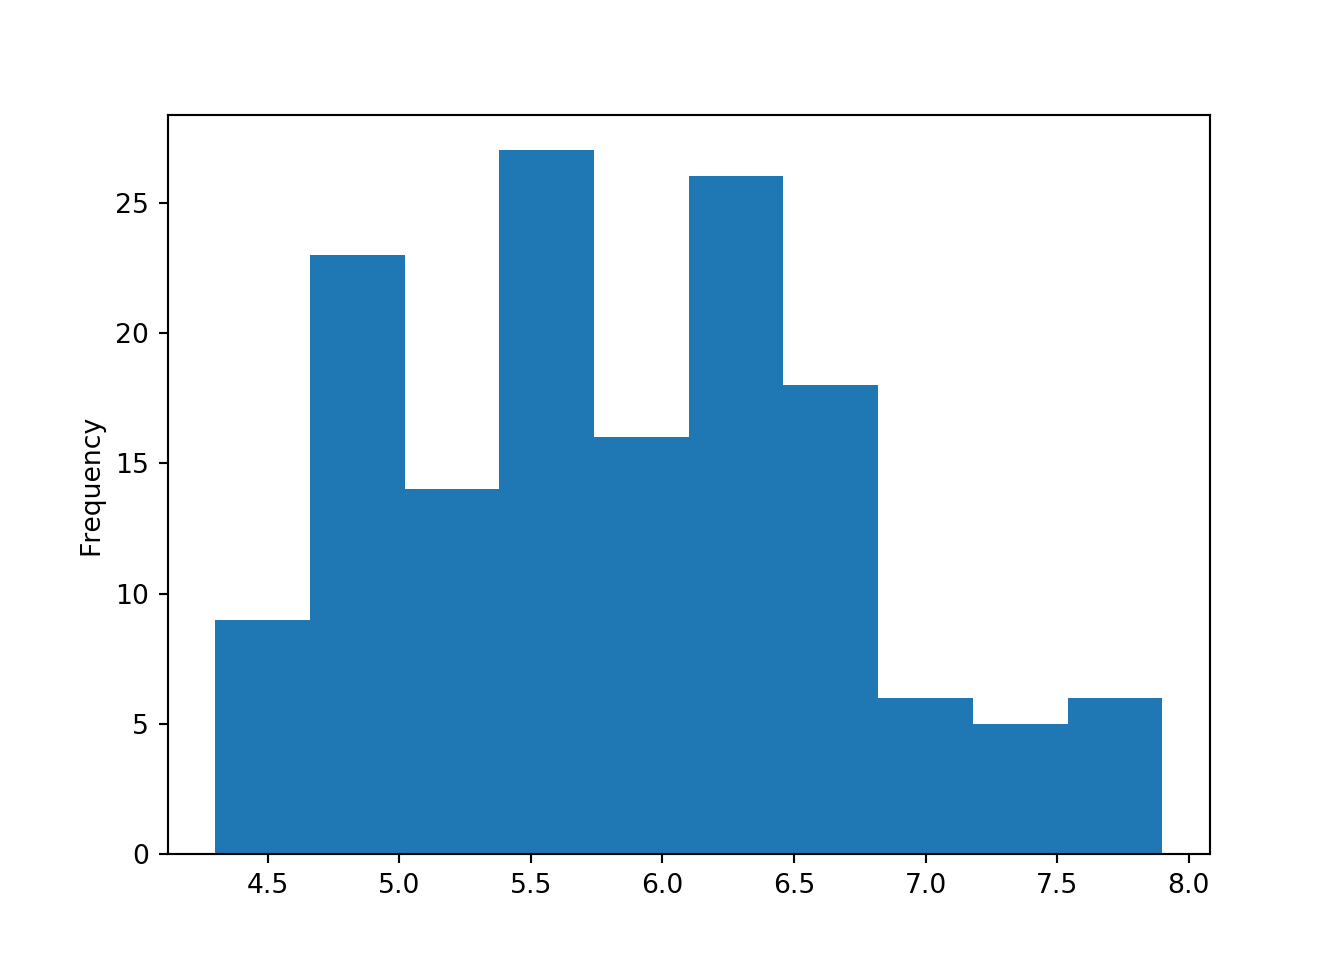
\includegraphics{Python_Documentation_files/figure-latex/unnamed-chunk-58-1.pdf}

\begin{Shaded}
\begin{Highlighting}[]
\NormalTok{cts }\OperatorTok{=}\NormalTok{ iris[}\StringTok{'species'}\NormalTok{].value_counts()}
\NormalTok{cts.plot(kind}\OperatorTok{=}\StringTok{'bar'}\NormalTok{)}
\NormalTok{plt.show()}
\end{Highlighting}
\end{Shaded}

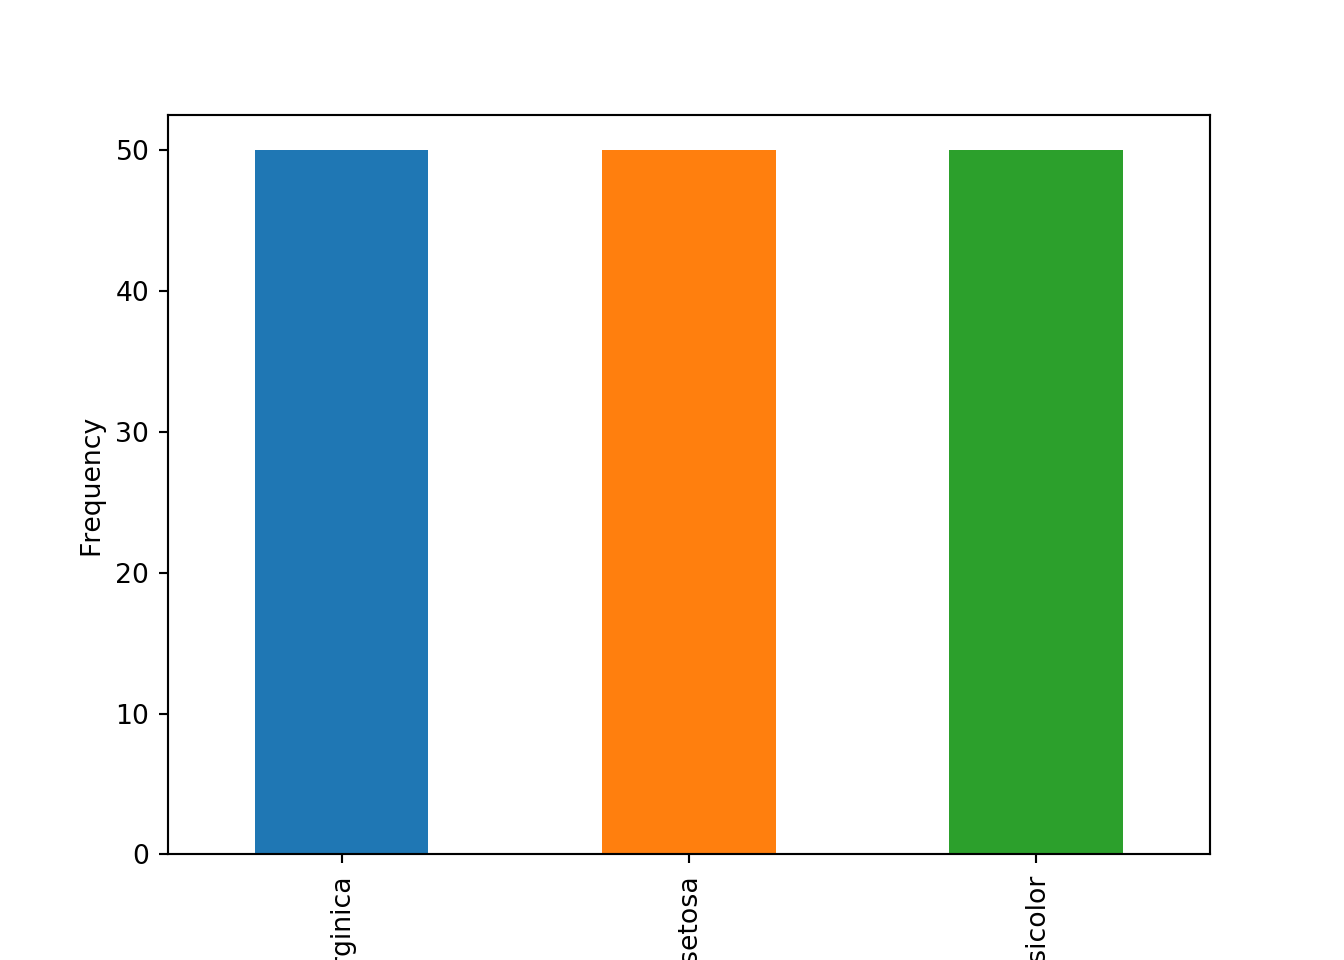
\includegraphics{Python_Documentation_files/figure-latex/unnamed-chunk-59-1.pdf}

\begin{Shaded}
\begin{Highlighting}[]
\NormalTok{iris.plot(kind}\OperatorTok{=}\StringTok{'scatter'}\NormalTok{, x}\OperatorTok{=}\StringTok{'sepal_length'}\NormalTok{, y}\OperatorTok{=}\StringTok{'sepal_width'}\NormalTok{)}
\NormalTok{plt.show()}
\end{Highlighting}
\end{Shaded}

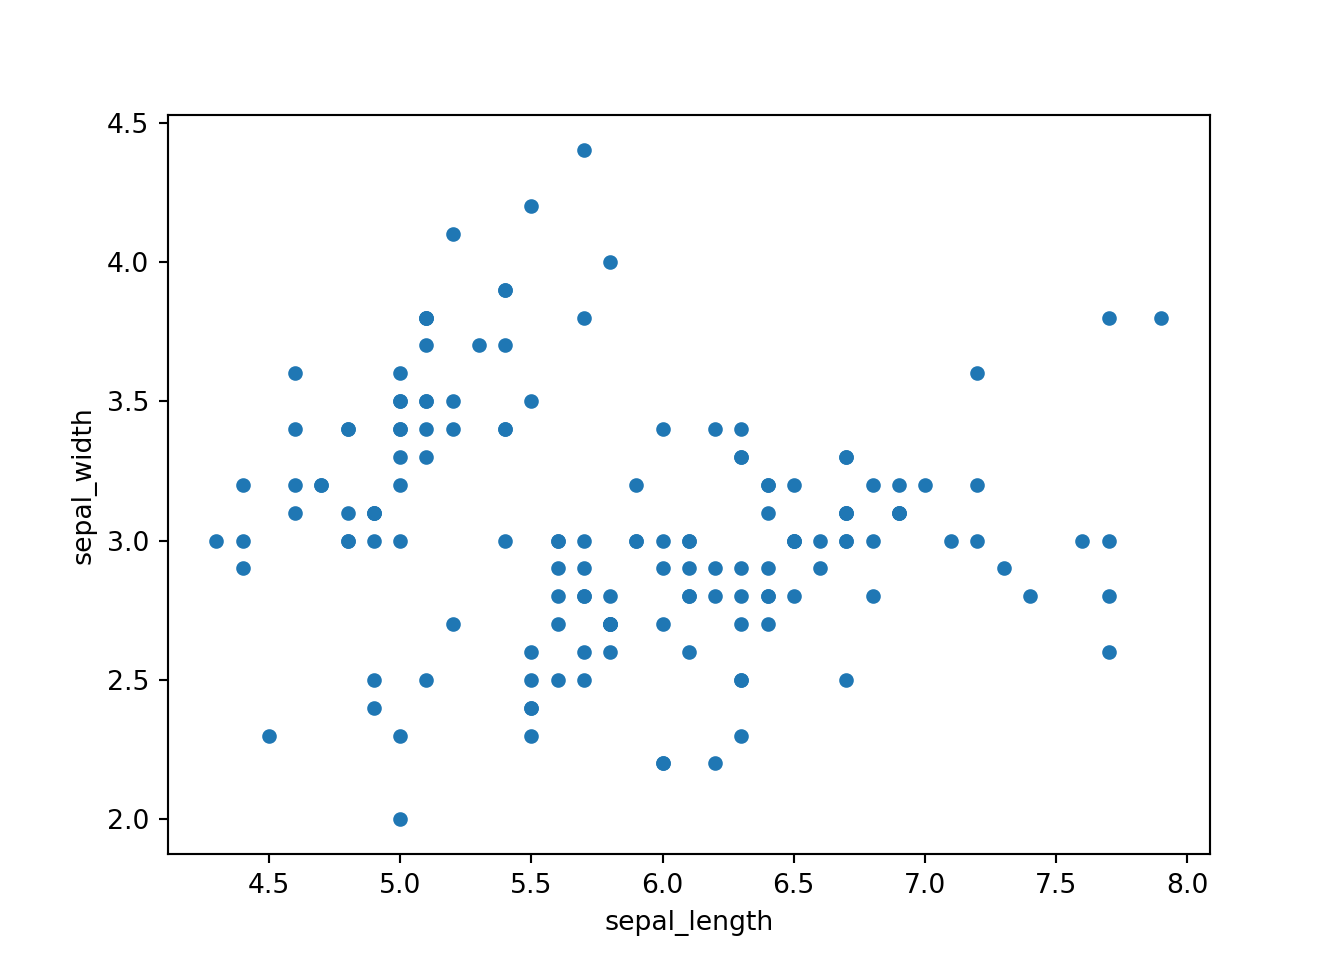
\includegraphics{Python_Documentation_files/figure-latex/unnamed-chunk-60-1.pdf}

\begin{Shaded}
\begin{Highlighting}[]
\NormalTok{iris.plot(kind}\OperatorTok{=}\StringTok{'box'}\NormalTok{)}
\NormalTok{plt.show()}
\end{Highlighting}
\end{Shaded}

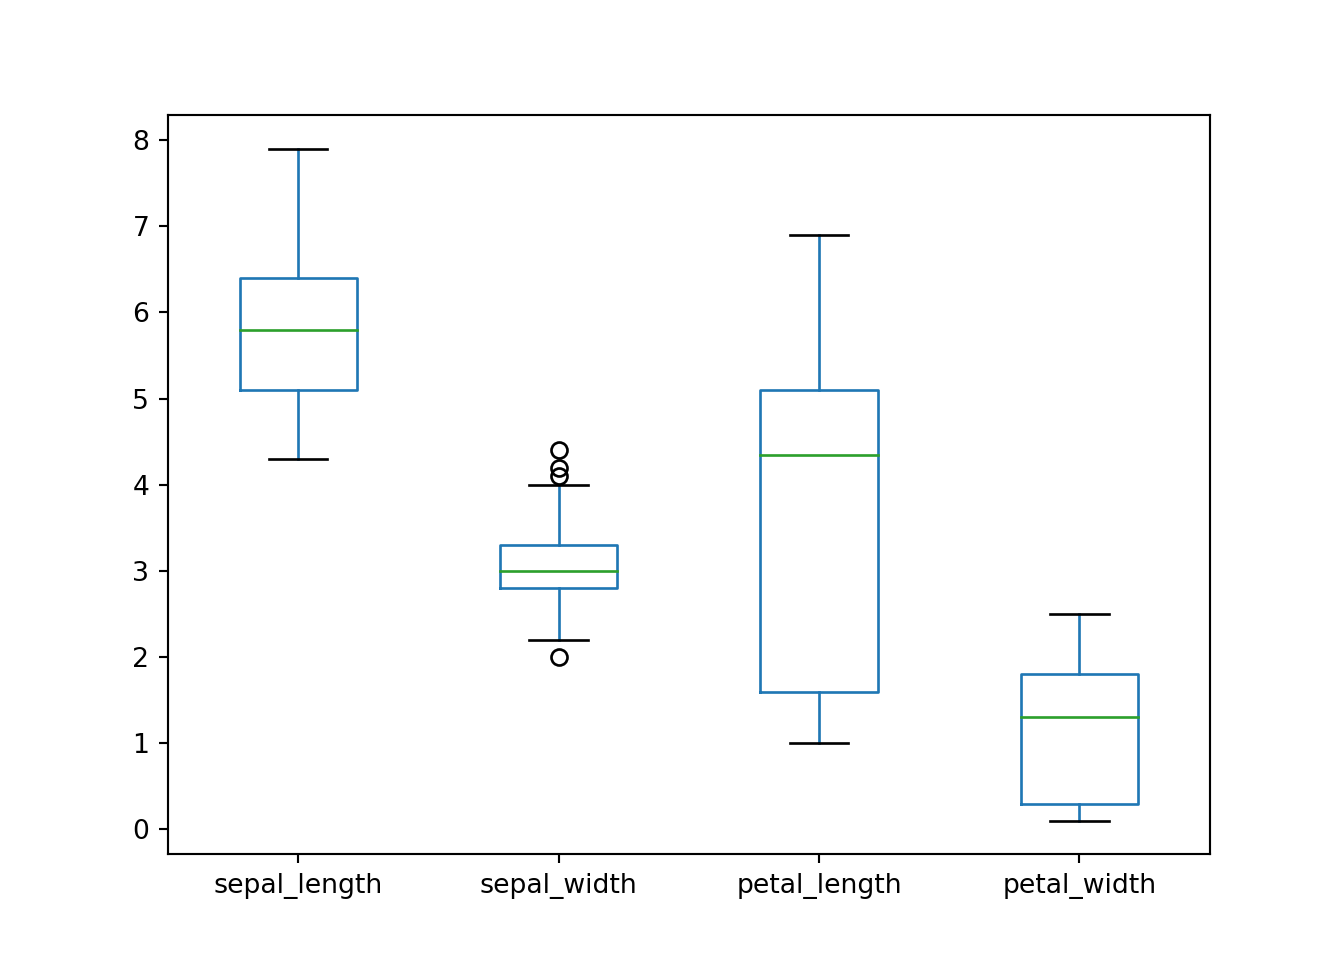
\includegraphics{Python_Documentation_files/figure-latex/unnamed-chunk-61-1.pdf}

\begin{Shaded}
\begin{Highlighting}[]
\NormalTok{iris.boxplot(by}\OperatorTok{=}\StringTok{'species'}\NormalTok{, column}\OperatorTok{=}\StringTok{'sepal_length'}\NormalTok{)}
\NormalTok{plt.show()}
\end{Highlighting}
\end{Shaded}

\hypertarget{data-visualization-with-seaborn}{%
\section{4.2 Data Visualization with
Seaborn}\label{data-visualization-with-seaborn}}

\begin{Shaded}
\begin{Highlighting}[]
\ImportTok{import}\NormalTok{ seaborn }\ImportTok{as}\NormalTok{ sns}
\ImportTok{import}\NormalTok{ matplotlib.pyplot }\ImportTok{as}\NormalTok{ plt}
\NormalTok{plt.clf()}
\NormalTok{sns.distplot(iris[}\StringTok{'sepal_length'}\NormalTok{])}
\NormalTok{plt.show()}
\end{Highlighting}
\end{Shaded}

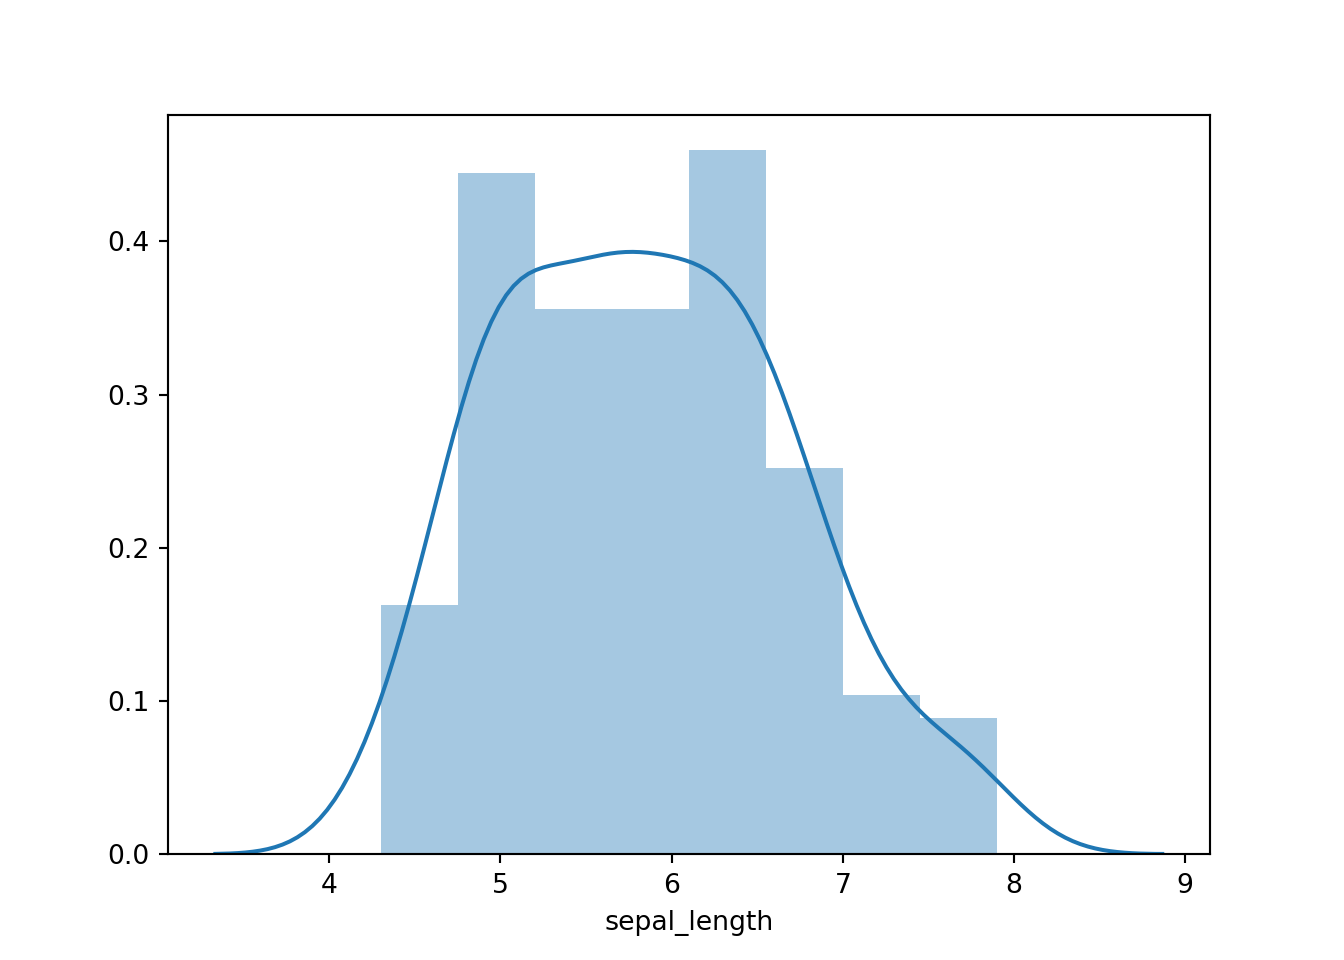
\includegraphics{Python_Documentation_files/figure-latex/unnamed-chunk-63-1.pdf}

Bar plot:No need to pretabulate the data:

\begin{Shaded}
\begin{Highlighting}[]
\NormalTok{sns.countplot(}\StringTok{'species'}\NormalTok{, data}\OperatorTok{=}\NormalTok{iris)}
\NormalTok{plt.show()}
\end{Highlighting}
\end{Shaded}

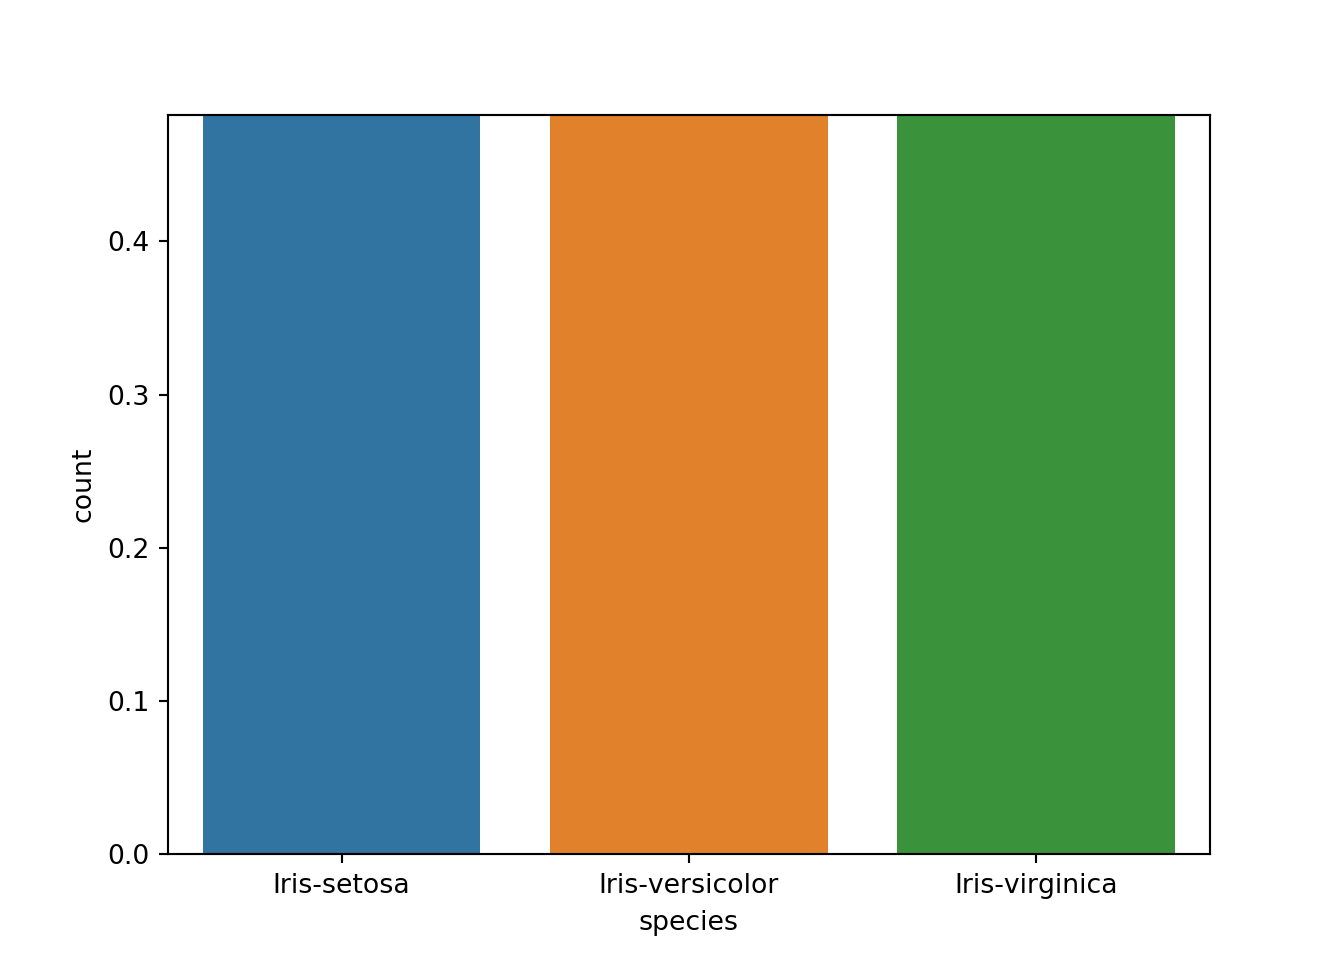
\includegraphics{Python_Documentation_files/figure-latex/unnamed-chunk-64-1.pdf}

Box plots:

\begin{Shaded}
\begin{Highlighting}[]
\NormalTok{sns.boxplot(x}\OperatorTok{=}\StringTok{'species'}\NormalTok{, y}\OperatorTok{=}\StringTok{'sepal_length'}\NormalTok{, data}\OperatorTok{=}\NormalTok{iris)}
\NormalTok{plt.show()}
\end{Highlighting}
\end{Shaded}

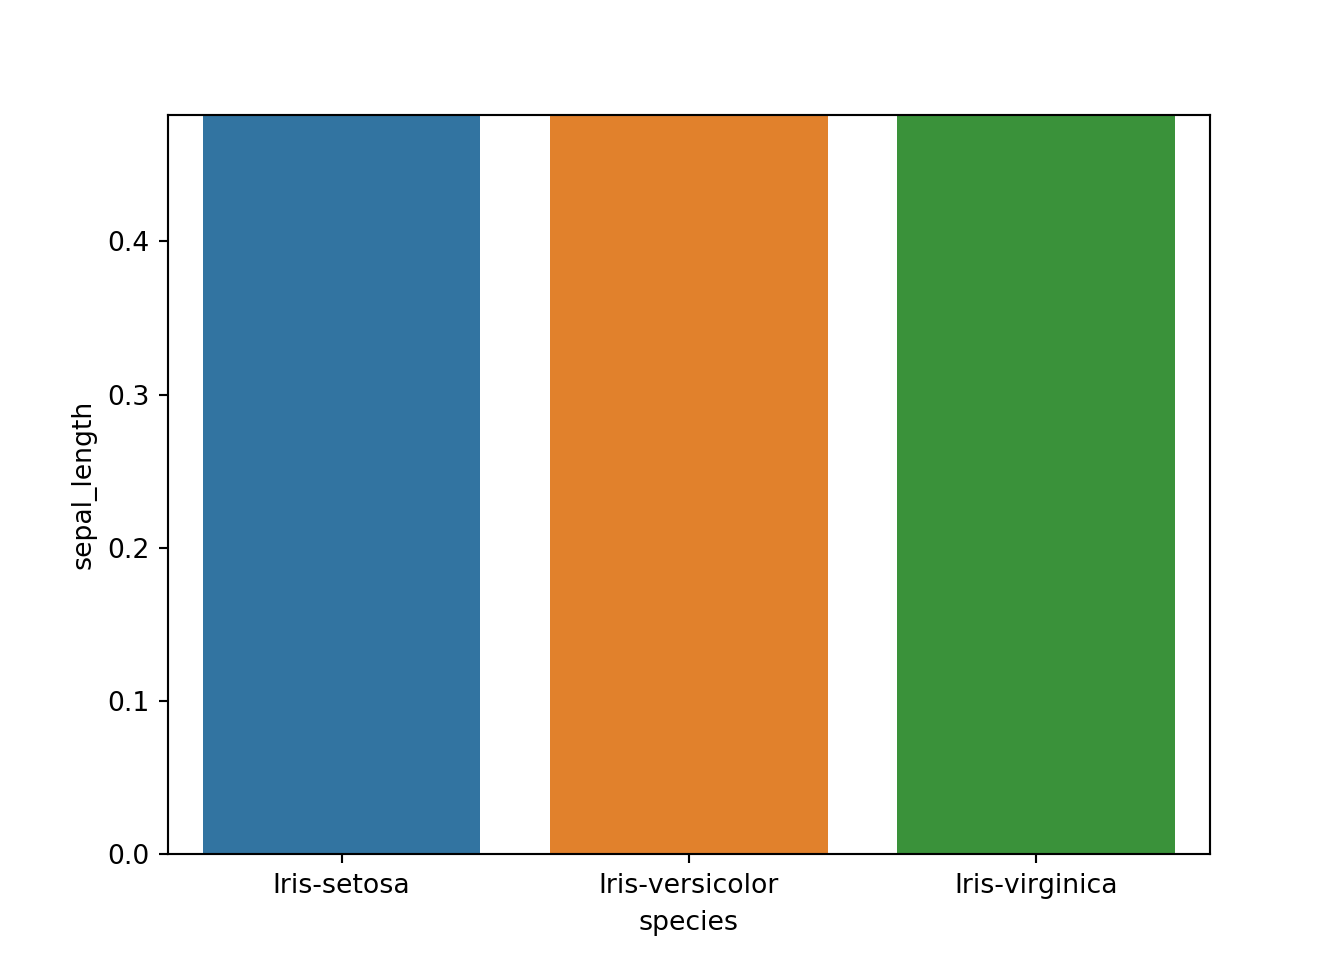
\includegraphics{Python_Documentation_files/figure-latex/unnamed-chunk-65-1.pdf}

regplot:

\begin{Shaded}
\begin{Highlighting}[]
\NormalTok{sns.regplot(x}\OperatorTok{=}\StringTok{'sepal_length'}\NormalTok{, y}\OperatorTok{=}\StringTok{'sepal_width'}\NormalTok{, data}\OperatorTok{=}\NormalTok{iris)}
\NormalTok{plt.show()}
\end{Highlighting}
\end{Shaded}

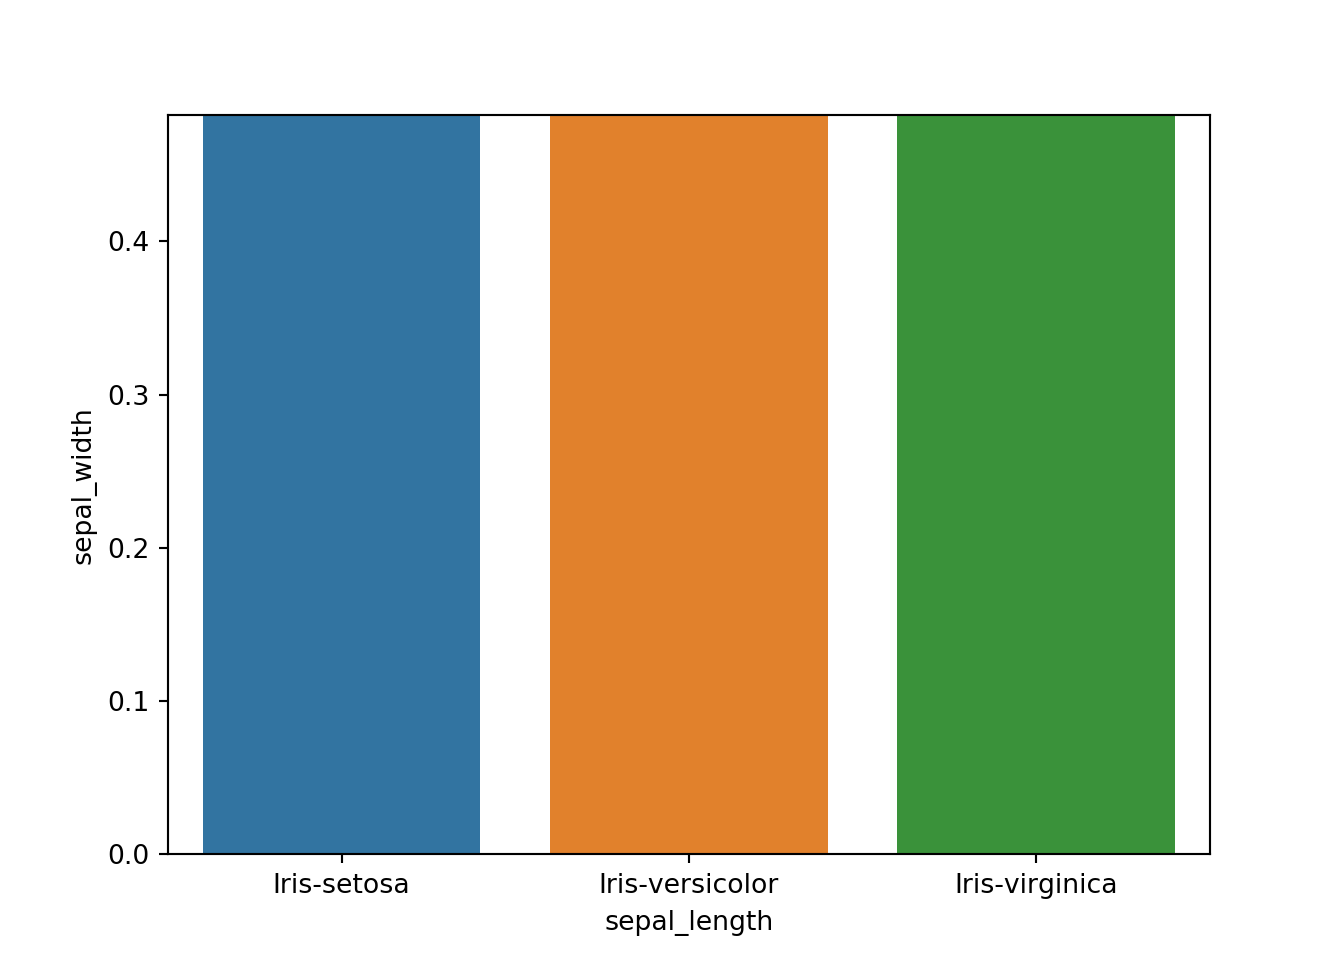
\includegraphics{Python_Documentation_files/figure-latex/unnamed-chunk-66-1.pdf}

No regression line:

\begin{Shaded}
\begin{Highlighting}[]
\NormalTok{sns.regplot(x}\OperatorTok{=}\StringTok{'sepal_length'}\NormalTok{, y}\OperatorTok{=}\StringTok{'sepal_width'}\NormalTok{, data}\OperatorTok{=}\NormalTok{iris,}
\NormalTok{            fit_reg}\OperatorTok{=}\VariableTok{False}\NormalTok{)}
\NormalTok{plt.show()}
\end{Highlighting}
\end{Shaded}

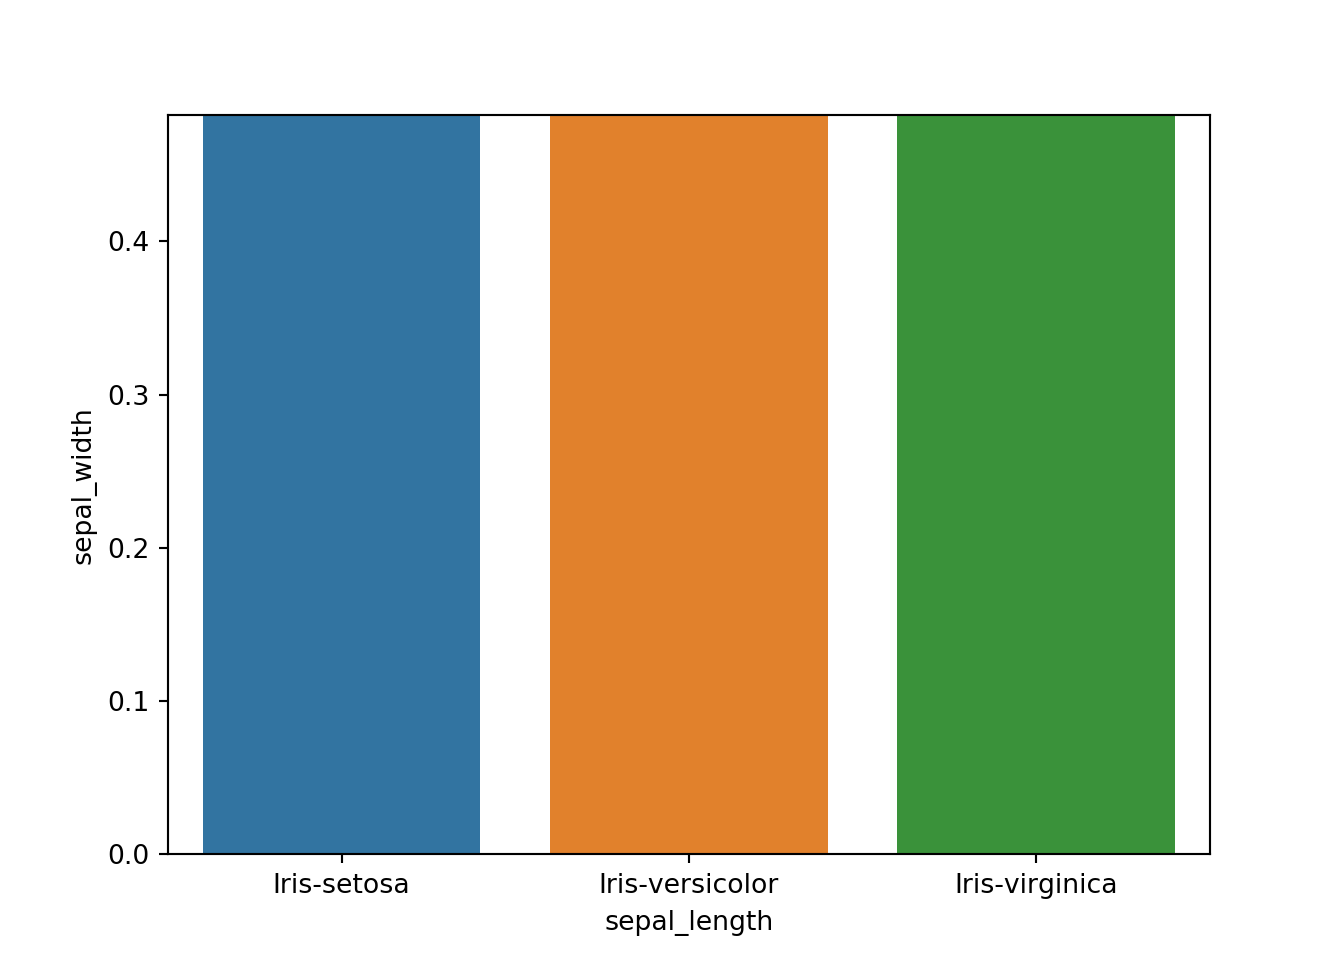
\includegraphics{Python_Documentation_files/figure-latex/unnamed-chunk-67-1.pdf}

Specify row and col arguments

\begin{Shaded}
\begin{Highlighting}[]
\NormalTok{sns.lmplot(x}\OperatorTok{=}\StringTok{'sepal_length'}\NormalTok{, y}\OperatorTok{=}\StringTok{'sepal_width'}\NormalTok{, data}\OperatorTok{=}\NormalTok{iris,}
\NormalTok{           fit_reg}\OperatorTok{=}\VariableTok{False}\NormalTok{,}
\NormalTok{           col}\OperatorTok{=}\StringTok{'species'}\NormalTok{)}
\NormalTok{plt.show()}
\end{Highlighting}
\end{Shaded}

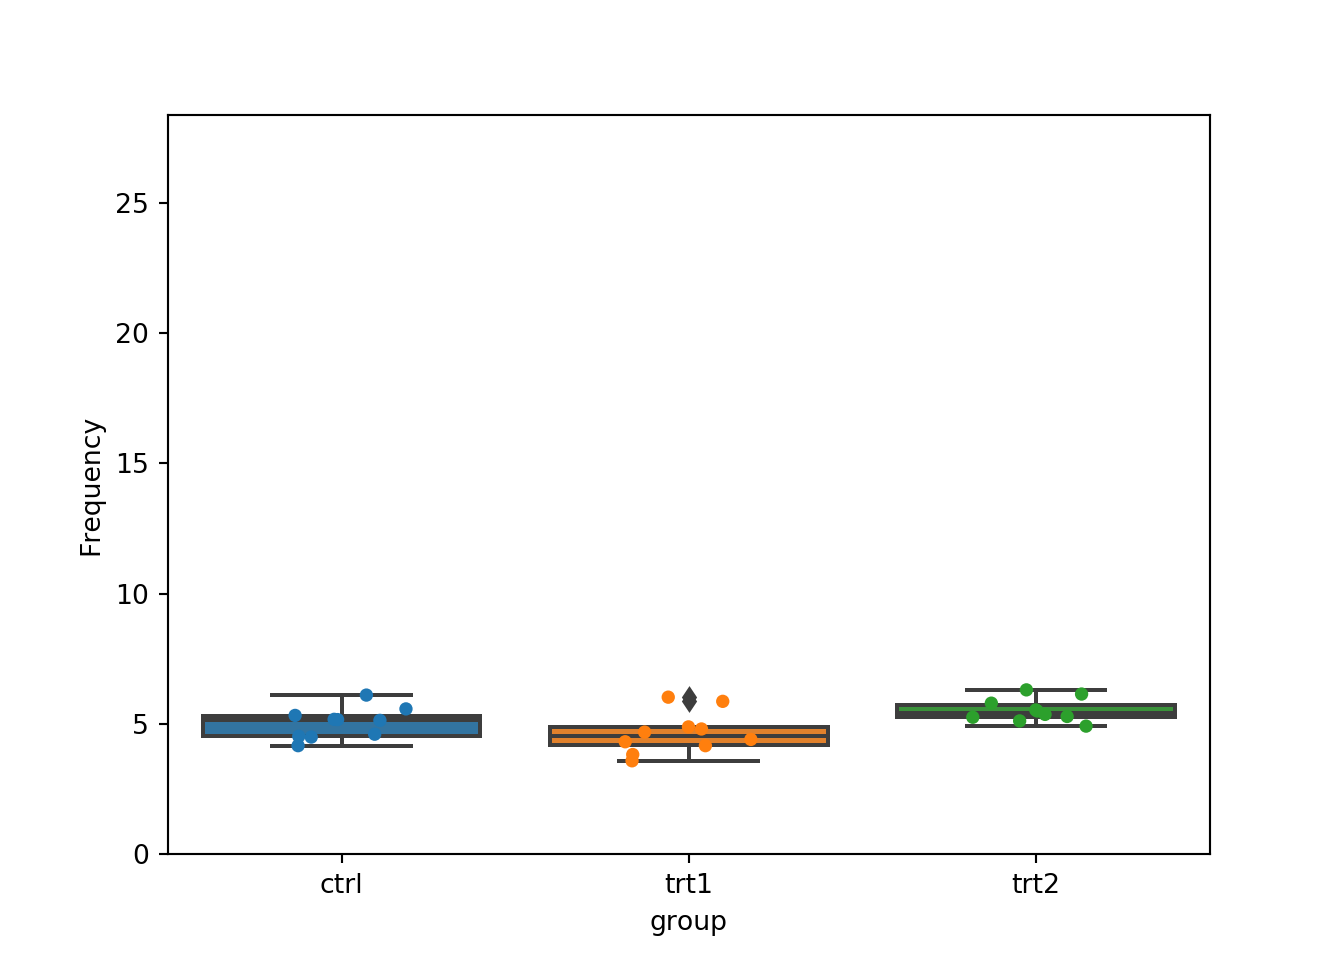
\includegraphics{Python_Documentation_files/figure-latex/unnamed-chunk-68-1.pdf}

Create a facet grid object and then map the plot into that.

\begin{Shaded}
\begin{Highlighting}[]
\NormalTok{g }\OperatorTok{=}\NormalTok{ sns.FacetGrid(iris, col}\OperatorTok{=}\StringTok{"species"}\NormalTok{)}
\NormalTok{g }\OperatorTok{=}\NormalTok{ g.}\BuiltInTok{map}\NormalTok{(plt.hist, }\StringTok{"sepal_length"}\NormalTok{)}
\NormalTok{plt.show()}
\end{Highlighting}
\end{Shaded}

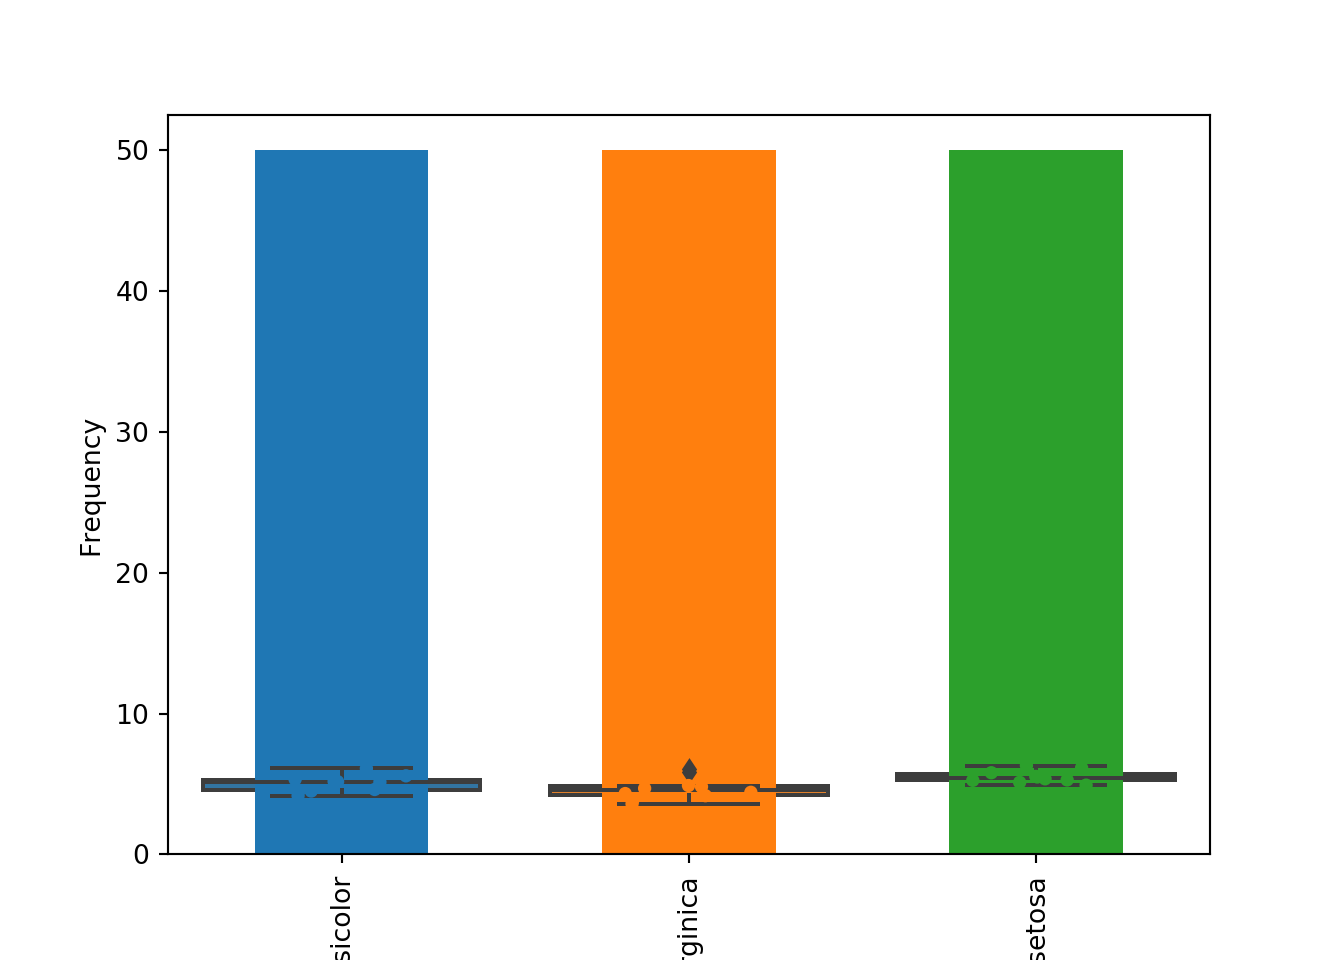
\includegraphics{Python_Documentation_files/figure-latex/unnamed-chunk-69-1.pdf}

g

\hypertarget{data-visualization-with-matplotlib}{%
\section{4.3 Data Visualization with
Matplotlib}\label{data-visualization-with-matplotlib}}

Histogram

\begin{Shaded}
\begin{Highlighting}[]
\ImportTok{import}\NormalTok{ matplotlib.pyplot }\ImportTok{as}\NormalTok{ plt}
\NormalTok{plt.clf()}
\NormalTok{plt.hist(iris[}\StringTok{'sepal_length'}\NormalTok{])}
\NormalTok{plt.show()}
\end{Highlighting}
\end{Shaded}

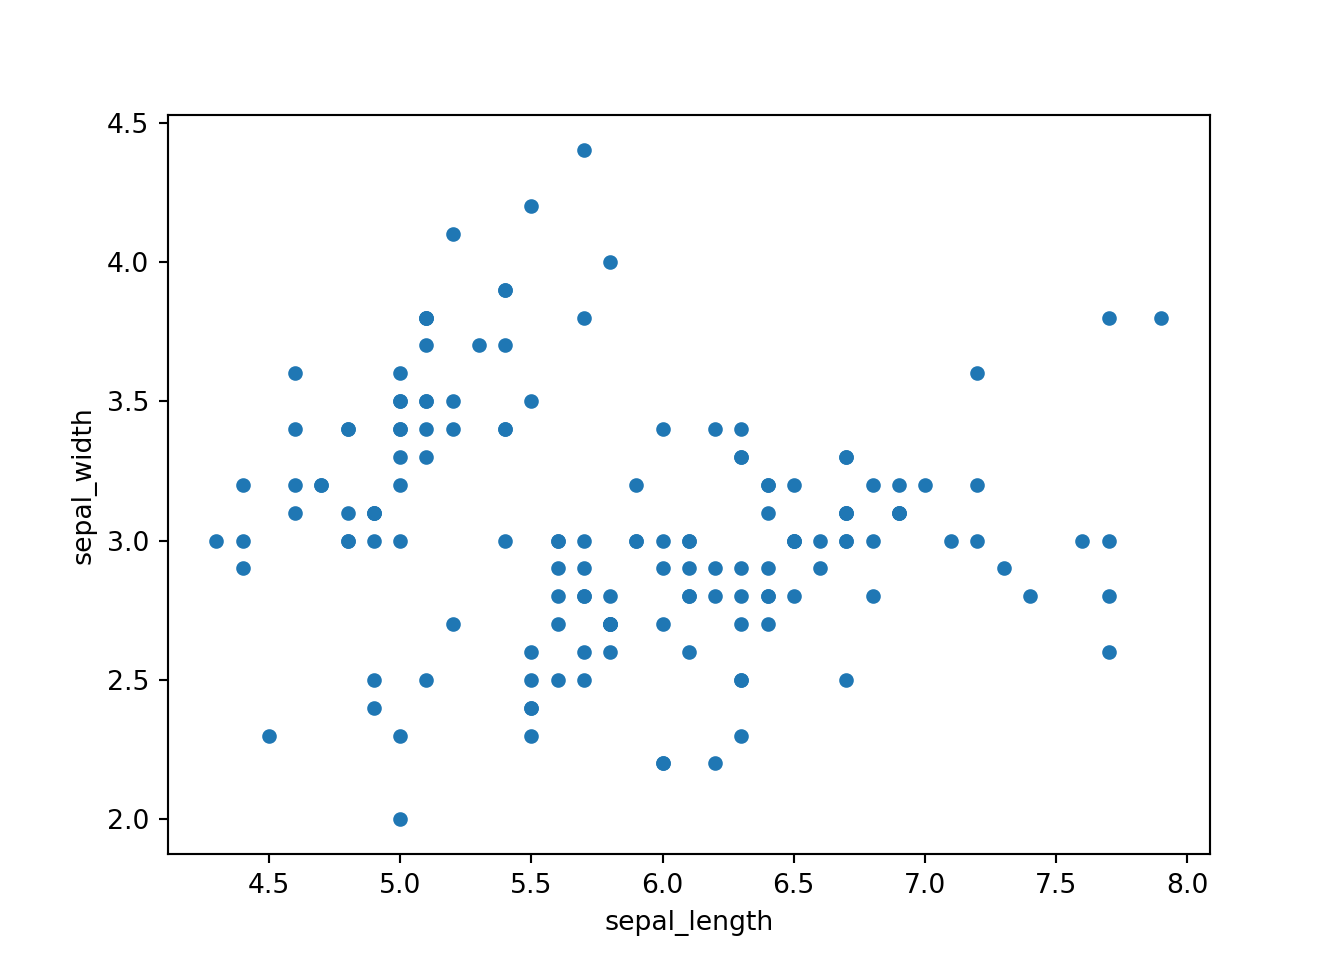
\includegraphics{Python_Documentation_files/figure-latex/unnamed-chunk-70-1.pdf}

Scatter plot

\begin{Shaded}
\begin{Highlighting}[]
\NormalTok{plt.clf()}
\NormalTok{plt.scatter(iris[}\StringTok{'sepal_length'}\NormalTok{], iris[}\StringTok{'sepal_width'}\NormalTok{])}
\NormalTok{plt.show()}
\end{Highlighting}
\end{Shaded}

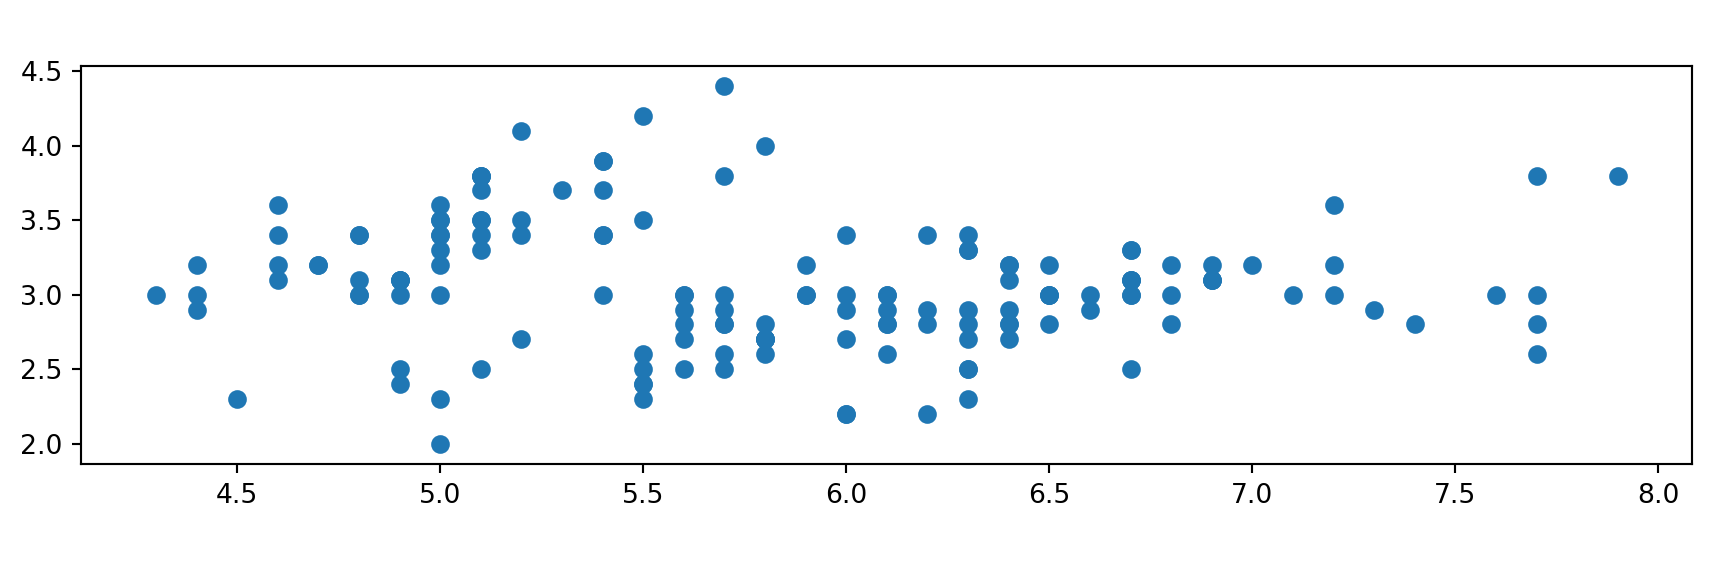
\includegraphics{Python_Documentation_files/figure-latex/unnamed-chunk-71-1.pdf}

\begin{Shaded}
\begin{Highlighting}[]
\NormalTok{fig, ax }\OperatorTok{=}\NormalTok{ plt.subplots()}
\NormalTok{ax.scatter(iris[}\StringTok{'sepal_length'}\NormalTok{], iris[}\StringTok{'sepal_width'}\NormalTok{])}
\NormalTok{ax.set_title(}\StringTok{'Sepal Length'}\NormalTok{)}
\NormalTok{ax.set_xlabel(}\StringTok{'Sepal Length'}\NormalTok{)}
\NormalTok{ax.set_ylabel(}\StringTok{'Sepal Width'}\NormalTok{)}
\NormalTok{plt.show()}
\end{Highlighting}
\end{Shaded}

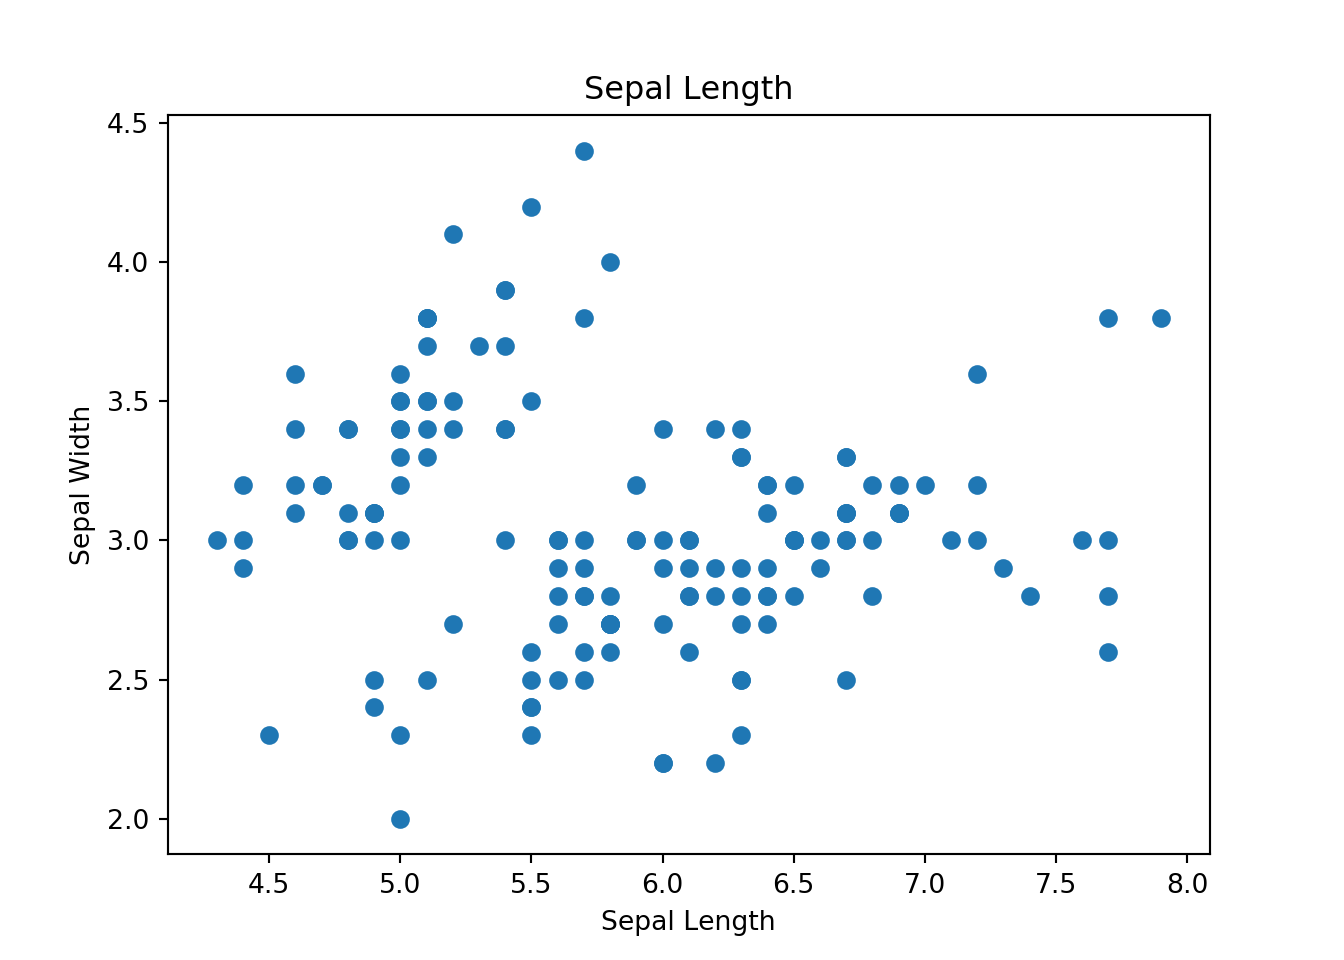
\includegraphics{Python_Documentation_files/figure-latex/unnamed-chunk-72-1.pdf}

\begin{Shaded}
\begin{Highlighting}[]
\NormalTok{fig, ax }\OperatorTok{=}\NormalTok{ plt.subplots()}
\NormalTok{ax.scatter(iris[}\StringTok{'sepal_length'}\NormalTok{], iris[}\StringTok{'sepal_width'}\NormalTok{])}
\NormalTok{ax.set_title(}\StringTok{'Sepal Length'}\NormalTok{)}
\NormalTok{ax.set_xlabel(}\StringTok{'Sepal Length'}\NormalTok{)}
\NormalTok{ax.set_ylabel(}\StringTok{'Sepal Width'}\NormalTok{)}
\NormalTok{plt.xticks(rotation}\OperatorTok{=}\DecValTok{45}\NormalTok{) }\CommentTok{# rotate the x-axis ticks}
\NormalTok{plt.show()}
\end{Highlighting}
\end{Shaded}

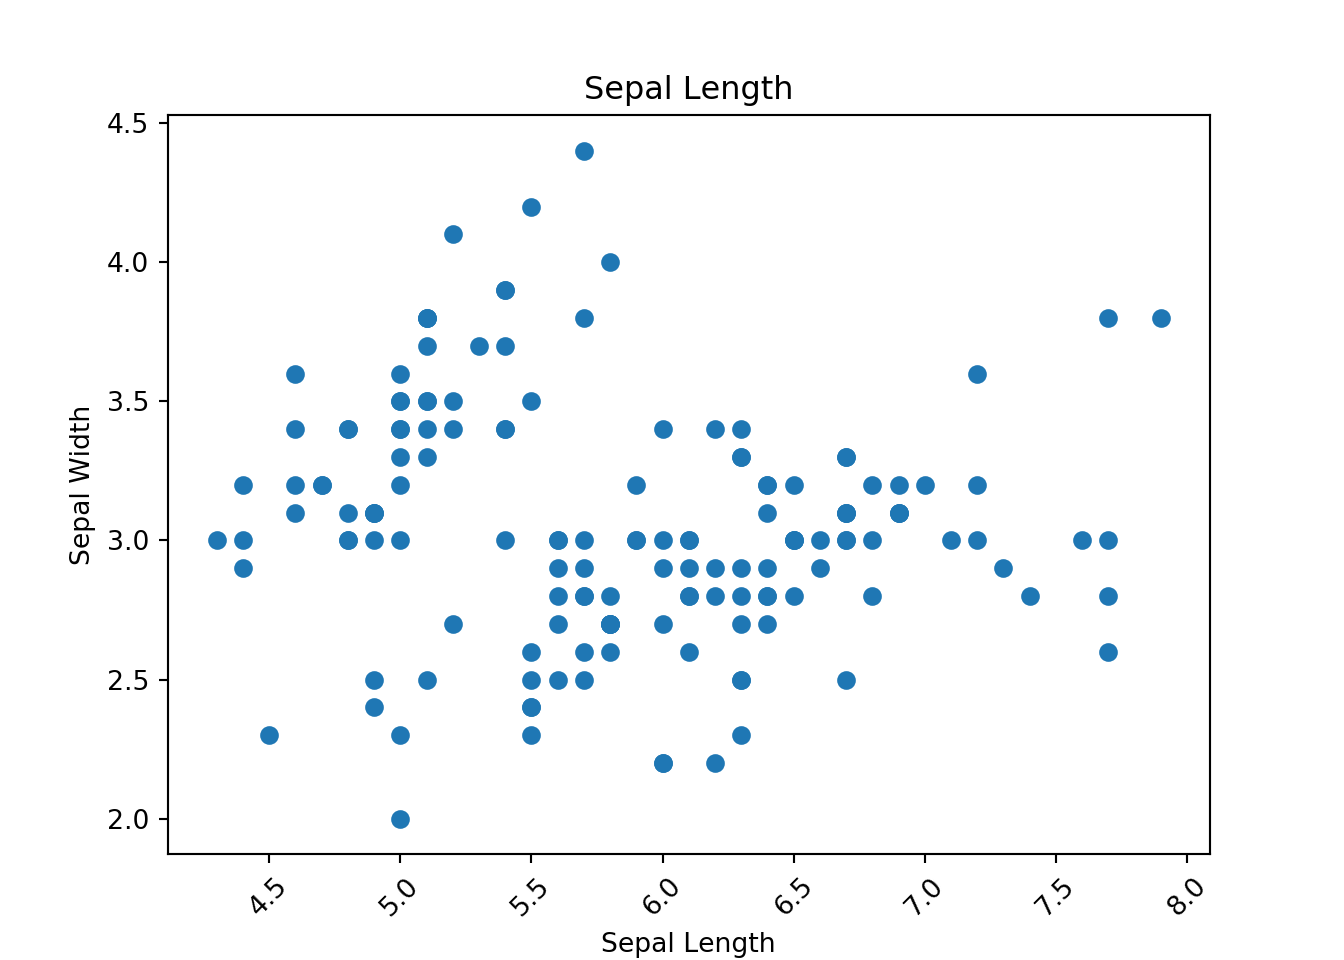
\includegraphics{Python_Documentation_files/figure-latex/unnamed-chunk-73-1.pdf}

The figure`
\texttt{fig\textasciigrave{}\textasciigrave{}\ is\ an\ entire\ image,\ but\ an\ Axes,}ax`,
is an individual plot in it, i.e.~sub plots.

we can call \texttt{scatter()} on the ax object.

\begin{Shaded}
\begin{Highlighting}[]
\NormalTok{fig, ax }\OperatorTok{=}\NormalTok{ plt.subplots()}
\NormalTok{ax.scatter(iris[}\StringTok{'sepal_length'}\NormalTok{], iris[}\StringTok{'sepal_width'}\NormalTok{])}
\NormalTok{plt.show()}
\end{Highlighting}
\end{Shaded}

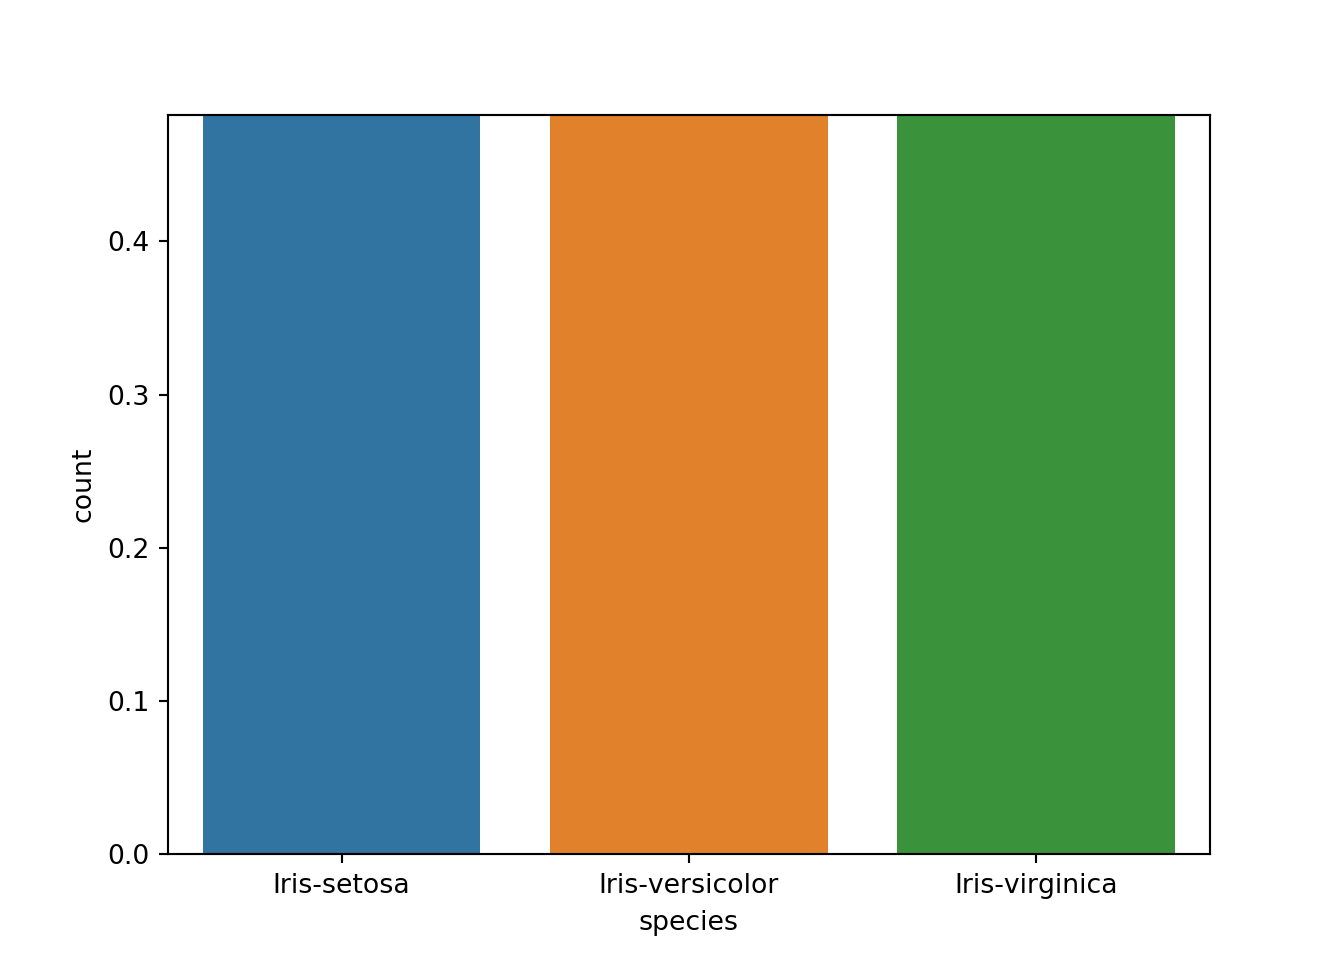
\includegraphics{Python_Documentation_files/figure-latex/unnamed-chunk-74-1.pdf}

Here we create two axes:

\begin{Shaded}
\begin{Highlighting}[]
\NormalTok{fig, (ax1, ax2) }\OperatorTok{=}\NormalTok{ plt.subplots(}\DecValTok{1}\NormalTok{, }\DecValTok{2}\NormalTok{)}
\NormalTok{ax1.scatter(iris[}\StringTok{'sepal_length'}\NormalTok{], iris[}\StringTok{'sepal_width'}\NormalTok{])}
\NormalTok{ax2.hist(iris[}\StringTok{'sepal_length'}\NormalTok{])}
\NormalTok{plt.show()}
\end{Highlighting}
\end{Shaded}

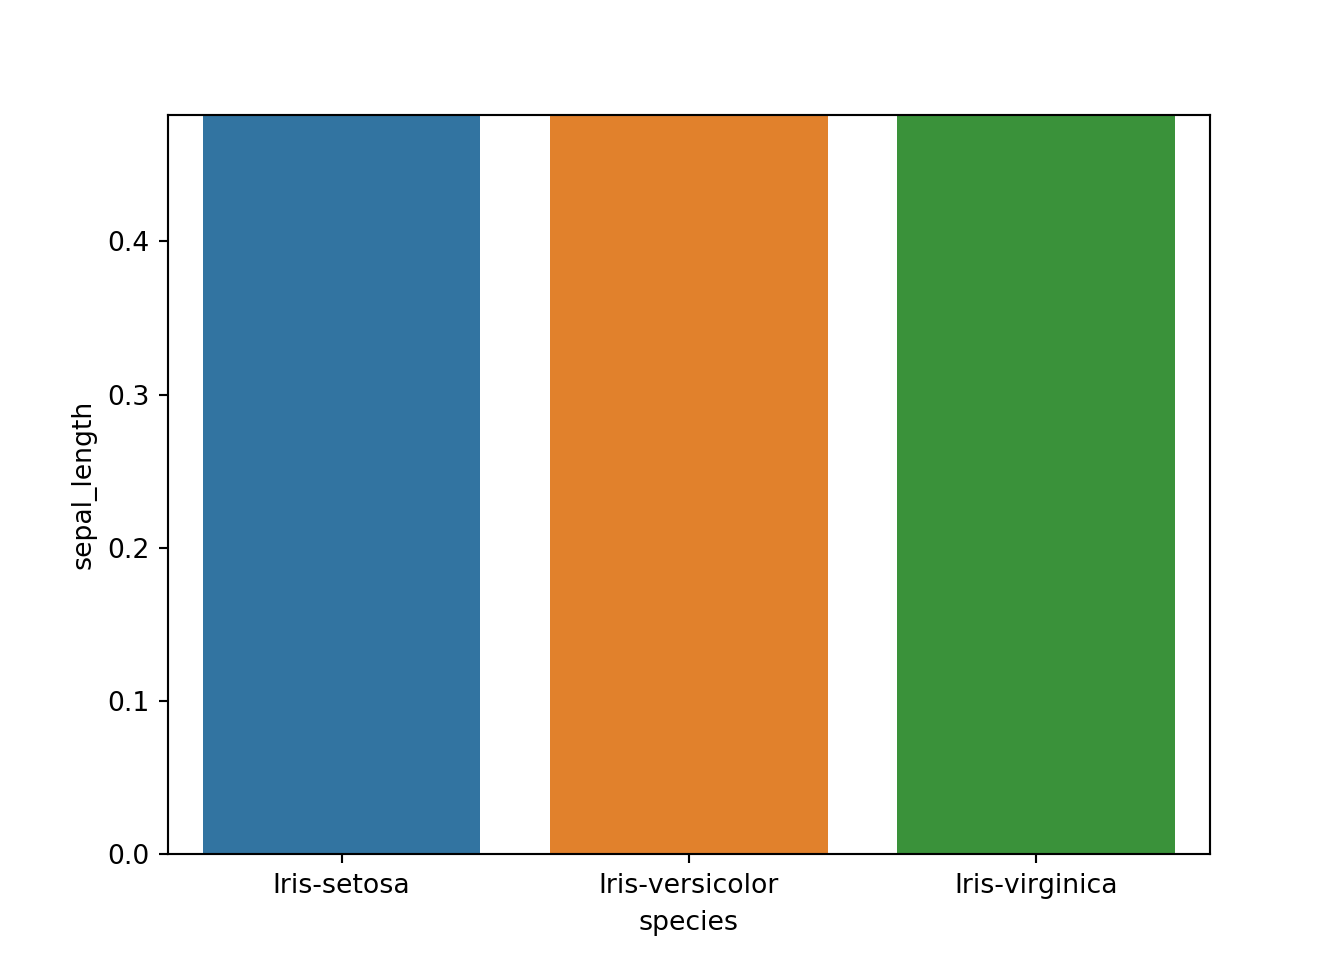
\includegraphics{Python_Documentation_files/figure-latex/unnamed-chunk-75-1.pdf}

You can mix functions form different plots: \texttt{ax\ =\ ax}

\begin{Shaded}
\begin{Highlighting}[]
\ImportTok{import}\NormalTok{ seaborn }\ImportTok{as}\NormalTok{ sns}
\NormalTok{fig, ax }\OperatorTok{=}\NormalTok{ plt.subplots()}
\NormalTok{sns.regplot(x}\OperatorTok{=}\StringTok{'sepal_length'}\NormalTok{, y}\OperatorTok{=}\StringTok{'sepal_width'}\NormalTok{,}
\NormalTok{            data}\OperatorTok{=}\NormalTok{iris, fit_reg}\OperatorTok{=}\VariableTok{False}\NormalTok{, ax}\OperatorTok{=}\NormalTok{ax)}
\NormalTok{plt.show()}
\end{Highlighting}
\end{Shaded}

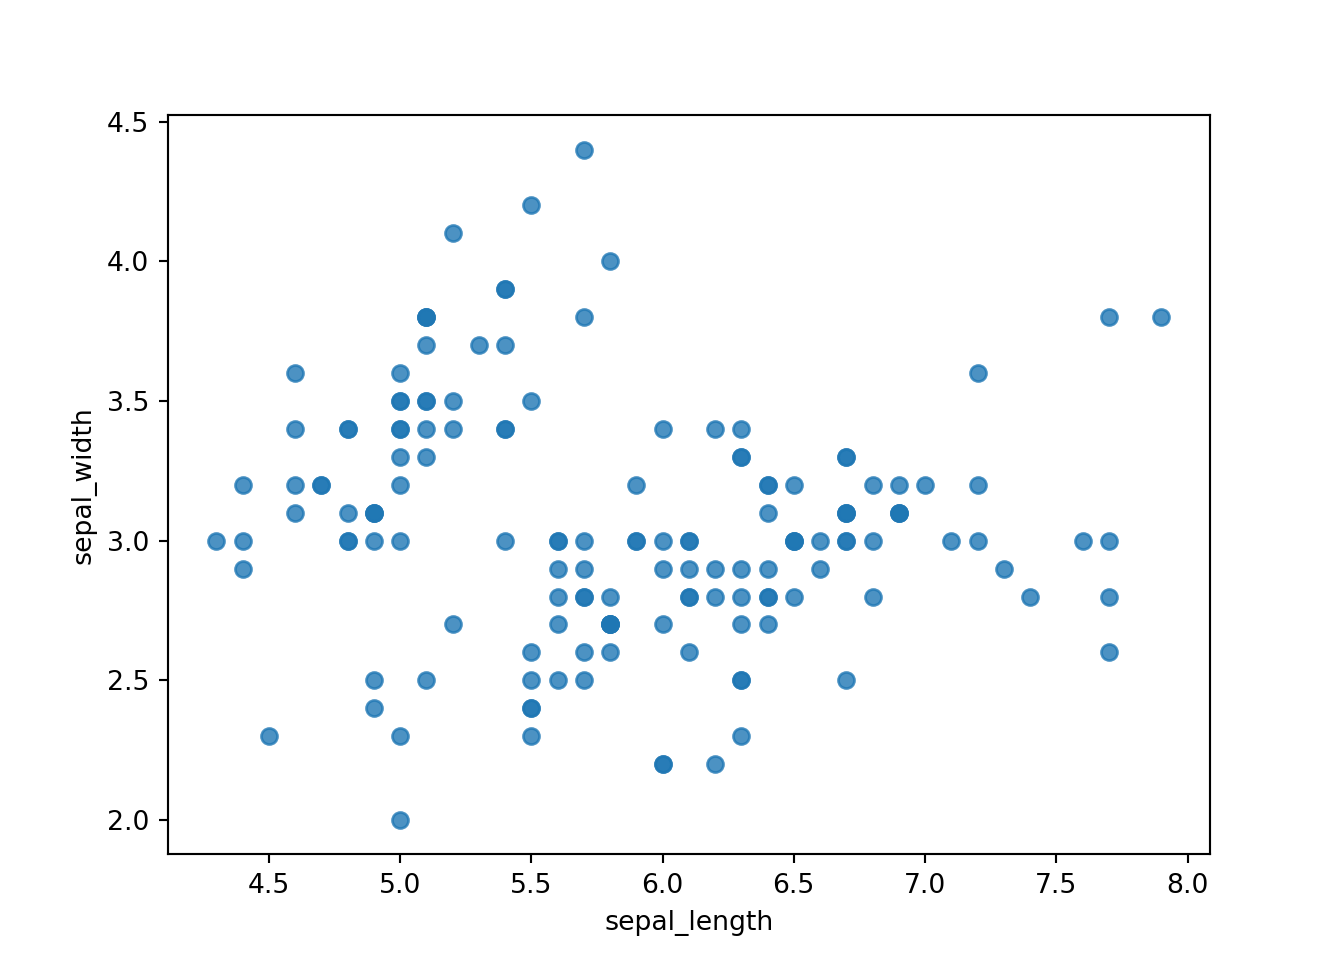
\includegraphics{Python_Documentation_files/figure-latex/unnamed-chunk-76-1.pdf}

Prevent plots from overlapping by clearing the figure with
\texttt{plt.clf()}.

\hypertarget{libraries-1}{%
\section{Libraries}\label{libraries-1}}

\hypertarget{numpy}{%
\subsection{Numpy}\label{numpy}}

Adds Python support for large, multi-dimensional arrays and matrices,
along with a large library of high-level mathematical functions to
operate on these arrays.

\hypertarget{scipy}{%
\subsection{SciPy}\label{scipy}}

A collection of mathematical algorithms and convenience functions built
on the Numpy extension of Python. It adds significant power to the
interactive Python session by providing the user with high-level
commands and classes for manipulating and visualizing data.

\hypertarget{pandas}{%
\subsection{Pandas}\label{pandas}}

Software library written for data manipulation and analysis in Python.
Offers data structures and operations for manipulating numerical tables
and time series.

\hypertarget{scikit-learn}{%
\subsection{Scikit-learn}\label{scikit-learn}}

A Python module for machine learning built on top of SciPy and
distributed under the 3-Clause BSD license.

\hypertarget{ch-5-virtualenv}{%
\chapter{Ch 5: virtualenv}\label{ch-5-virtualenv}}

\hypertarget{setting-up-your-virtual-env}{%
\section{Setting up your virtual
env}\label{setting-up-your-virtual-env}}

\begin{verbatim}
virtualenv ~/ds_intro -p /anaconda3/bin/python3.6
python -V

source ~/ds_intro/bin/activate
pip install pandas
pip install sklearn
pip install scipy
pip install jupyter

pip install seaborn
atom
pip install mpl_toolkits
pip install sympy
deactivate
\end{verbatim}

Connect to shiny server

\begin{verbatim}
ssh -i .ssh/Rick2018.pem ubuntu@ec2-18-185-131-255.eu-central-1.compute.amazonaws.com
\end{verbatim}

on server

\begin{verbatim}
sudo -i
\end{verbatim}

As root user, install packages

\begin{verbatim}
sudo su - -c "R -e \"install.packages('shiny', repos='http://cran.rstudio.com/')\""
\end{verbatim}

\bibliography{book.bib,packages.bib}


\end{document}
